% Task C23
% Source volume: lower
% Physical scan pages: 291--320
% Printed book pages: 279--308
% Transcribe only source content; omit running headers, footers, and printed page numbers.
\chapter{含参变量积分}

% BEGIN TRANSCRIPTION

在 §23.1 和 §23.2 两节中考虑含参变量积分的一般性质，其中包括含参变量常义积分和含参变量广义积分。对后者而言，其分析性质的研究首先涉及这些广义积分的收敛性是否关于参变量一致。然后给出许多具体计算的例子。在 §23.3 中介绍两个重要的特殊函数：B 函数和 $\Gamma$ 函数。最后一节是学习要点和参考题。

\section{含参变量常义积分}

\subsection{定义与性质}

在实际问题中我们经常会遇到带参数的积分，比如椭圆
\[
  \frac{x^2}{a^2}+\frac{y^2}{b^2}=1\qquad (b>a>0)
\]
的弧长为
\[
  l=4\int_0^{\pi/2}\sqrt{a^2\sin^2 t+b^2\cos^2 t}\,\dd t
  =4b\int_0^{\pi/2}\sqrt{1-k^2\sin^2 t}\,\dd t,
\]
其中 $k=\dfrac{\sqrt{b^2-a^2}}{b}$ 是离心率。这里
\[
  I(k)=\int_0^{\pi/2}\sqrt{1-k^2\sin^2 t}\,\dd t
\]
称为第二类完全椭圆积分，它不能用初等函数表示\footnote{关于椭圆弧长以及椭圆积分参见上册 356 页和第十六章例题 16.1.1。}。$I(k)$ 就是含参变量积分的一个例子。一般地，设 $D\subset\RR$，二元函数 $f(x,t)$ 定义在 $[a,b]\times D$ 上，$\forall t\in D$，设 $f(x,t)$ 作为 $x$ 的函数在 $[a,b]$ 上常义可积，即通常所说的有界可积，则
\[
  \varphi(t)=\int_a^b f(x,t)\,\dd x
\]
是定义在 $D$ 上的含参变量常义积分。它具有如下主要性质。

\begin{xproposition}[23.1.1（极限性质）]
设 $t_0$ 是 $D$ 的聚点，如果 $\lim\limits_{t\to t_0}f(x,t)=\psi(x)$，且收敛关于 $x\in[a,b]$ 是一致的，则 $\psi(x)$ 在 $[a,b]$ 上有界可积，且
\[
  \lim_{t\to t_0}\varphi(t)
  =\lim_{t\to t_0}\int_a^b f(x,t)\,\dd x
  =\int_a^b\psi(x)\,\dd x.
\]
\end{xproposition}

\begin{xproposition}[23.1.2（连续性）]
设 $f(x,t)$ 在 $[a,b]\times[c,d]$ 上连续，则
\[
  \varphi(t)=\int_a^b f(x,t)\,\dd x
\]
在 $[c,d]$ 上连续。
\end{xproposition}

\begin{xproposition}[23.1.3（交换积分次序）]
设 $f(x,t)$ 在 $[a,b]\times[c,d]$ 上连续，则
\[
  \int_c^d\dd t\int_a^b f(x,t)\,\dd x
  =\int_a^b\dd x\int_c^d f(x,t)\,\dd t.
\]
\end{xproposition}

\begin{xproposition}[23.1.4（可微性）]
设 $f(x,t)$，$f_t(x,t)$ 在 $[a,b]\times[c,d]$ 上连续，则
\[
  \varphi(t)=\int_a^b f(x,t)\,\dd x
\]
在 $[c,d]$ 上可导，且
\[
  \varphi'(t)=\int_a^b f_t(x,t)\,\dd x.
\]
\end{xproposition}

如果在积分限中也含有参变量，则我们有如下更一般的结论。

\begin{xproposition}[23.1.5]
设 $f(x,t)$ 在 $[a,b]\times[c,d]$ 上连续，$\alpha(t)$ 和 $\beta(t)$ 都在 $[c,d]$ 上连续，且
\[
  a\leqslant \alpha(t),\beta(t)\leqslant b,\qquad \forall t\in[c,d],
\]
则
\[
  \varphi(t)=\int_{\alpha(t)}^{\beta(t)}f(x,t)\,\dd x
\]
在 $[c,d]$ 上连续。进一步若 $f_t(x,t)$ 也在 $[a,b]\times[c,d]$ 上连续，$\alpha(t)$ 和 $\beta(t)$ 都在 $[c,d]$ 上可导，则 $\varphi(t)$ 也在 $[c,d]$ 上可导，且
\[
  \varphi'(t)=f(\beta(t),t)\beta'(t)-f(\alpha(t),t)\alpha'(t)
  +\int_{\alpha(t)}^{\beta(t)}f_t(x,t)\,\dd x.
\]
\end{xproposition}

\begin{xexample}[23.1.1]
设 $f(x)$ 在 $[0,1]$ 上连续，考察函数
\[
  F(t)=\int_0^1\frac{t}{x^2+t^2}f(x)\,\dd x
\]
的连续性。
\end{xexample}
\begin{xsolution}
显然 $F(t)$ 定义在 $(-\infty,+\infty)$ 上且 $\forall t_0\neq0$，$h(x,t)=\dfrac{tf(x)}{x^2+t^2}$ 在 $[0,1]\times[\frac12t_0,2t_0]$ 上连续（或在 $[0,1]\times[2t_0,\frac12t_0]$ 上连续），由命题 23.1.2 知 $F(t)$ 在 $t_0$ 点连续。

下面讨论 $F(t)$ 在 $t=0$ 处的连续性。我们先考虑
\[
  \lim_{t\to0^+}F(t)=\lim_{t\to0^+}\int_0^1\frac{t}{x^2+t^2}f(x)\,\dd x.
\]
注意到
\[
  \int_0^1\frac{t}{x^2+t^2}f(x)\,\dd x
  =\int_0^{t^{1/3}}\frac{t}{x^2+t^2}f(x)\,\dd x
  +\int_{t^{1/3}}^1\frac{t}{x^2+t^2}f(x)\,\dd x.
\]
而当 $t\to0^+$ 时，
\[
  \int_0^{t^{1/3}}\frac{t}{x^2+t^2}f(x)\,\dd x
  =f(\xi)\arctan\frac{t^{1/3}}{t}\to f(0)\frac{\pi}{2},
\]
\[
  \left|\int_{t^{1/3}}^1\frac{t}{x^2+t^2}f(x)\,\dd x\right|
  \leqslant \max_{0\leqslant x\leqslant1}\{|f(x)|\}\cdot
  \frac{t}{t^{2/3}+t^2}\to0.
\]
因此
\[
  \lim_{t\to0^+}\int_0^1\frac{t}{x^2+t^2}f(x)\,\dd x=f(0)\frac{\pi}{2}.
\]
同理可证
\[
  \lim_{t\to0^-}F(t)=-f(0)\frac{\pi}{2},
\]
所以当 $f(0)=0$ 时，$F(t)$ 在点 $t=0$ 处连续；否则在该点处不连续。
\end{xsolution}

\begin{xexample}[23.1.2]
设
\[
  F(t)=\int_0^{t^2}\dd x\int_{x-t}^{x+t}\sin(x^2+y^2-t^2)\,\dd y,
\]
求 $F'(t)$。
\end{xexample}
\begin{xsolution}
令
\[
  f(x,t)=\int_{x-t}^{x+t}\sin(x^2+y^2-t^2)\,\dd y,
\]
其中 $x,t$ 为参变量。由含参变量积分的求导公式
\[
  F'(t)=2t\int_{t^2-t}^{t^2+t}\sin(t^4+y^2-t^2)\,\dd y
  +\int_0^{t^2}\left(\frac{\partial}{\partial t}
  \int_{x-t}^{x+t}\sin(x^2+y^2-t^2)\,\dd y\right)\dd x.
\]
而
\[
\begin{aligned}
  \frac{\partial}{\partial t}\int_{x-t}^{x+t}\sin(x^2+y^2-t^2)\,\dd y
  ={}&\sin[x^2+(x+t)^2-t^2]-(-1)\sin[x^2+(x-t)^2-t^2]\\
  &+\int_{x-t}^{x+t}(-2t)\cos(x^2+y^2-t^2)\,\dd y\\
  ={}&2\sin2x^2\cos2xt-2t\int_{x-t}^{x+t}\cos(x^2+y^2-t^2)\,\dd y.
\end{aligned}
\]
最后得到
\[
\begin{aligned}
  F'(t)={}&2t\int_{t^2-t}^{t^2+t}\sin(t^4+y^2-t^2)\,\dd y
  +2\int_0^{t^2}\sin2x^2\cos2xt\,\dd x\\
  &-2t\int_0^{t^2}\dd x\int_{x-t}^{x+t}\cos(x^2+y^2-t^2)\,\dd y.
\end{aligned}
\]
\end{xsolution}

\subsection{几种常用的求参变量积分的方法}

如果直接求
\[
  \varphi(t)=\int_a^b f(x,t)\,\dd x
\]
有困难，常采用以下两种方法：
\begin{enumerate}
  \item 先求 $\varphi'(t)$，即先求 $\displaystyle\int_a^b f_t(x,t)\,\dd x$，然后再对 $t$ 积分求出 $\varphi(t)$。
  \item 把 $f(x,t)$ 表示为积分形式，再用积分号下求积分的方法。此时通常要交换积分次序。
\end{enumerate}

\begin{xexample}[23.1.3]
计算
\begin{equation}
  I(x)=\int_0^{\pi/2}\ln(\sin^2\theta+x^2\cos^2\theta)\,\dd\theta,
  \qquad 0<x<+\infty.
  \tag{23.1}
  \label{eq:23.1}
\end{equation}
\end{xexample}
\begin{xsolution}
令 $f(x,\theta)=\ln(\sin^2\theta+x^2\cos^2\theta)$，$\forall x_0\in(0,+\infty)$，$f(x,\theta)$ 在 $[\frac12x_0,2x_0]\times[0,\frac\pi2]$ 上连续，且
\[
  f_x(x,\theta)=\frac{2x\cos^2\theta}{\sin^2\theta+x^2\cos^2\theta}
\]
也在 $[\frac12x_0,2x_0]\times[0,\frac\pi2]$ 上连续。应用积分号下求导的性质，可得 $\forall x\in(0,+\infty)$，
\[
\begin{aligned}
  I'(x)
  &=\int_0^{\pi/2}\frac{2x\cos^2\theta}{\sin^2\theta+x^2\cos^2\theta}\,\dd\theta
   =2x\int_0^{\pi/2}\frac{\dd\theta}{x^2+\tan^2\theta}\qquad(\text{令 }\tan\theta=t)\\
  &=2x\int_0^{+\infty}\frac{1}{x^2+t^2}\cdot\frac{1}{1+t^2}\,\dd t\\
  &=\frac{2x}{x^2-1}\int_0^{+\infty}
  \left(\frac{1}{1+t^2}-\frac{1}{x^2+t^2}\right)\dd t\qquad(x\neq1)\\
  &=\frac{2x}{x^2-1}\left(\frac\pi2-\frac1x\frac\pi2\right)
  =\frac{\pi}{1+x}.
\end{aligned}
\]
积分得
\[
  I(x)=\pi\ln(1+x)+C\qquad(x\neq1).
\]
由 $I(x)$ 的连续性知上述表达式对 $x=1$ 也成立。在 (23.1) 中，令 $x=1$，则 $I(1)=0$，从而 $C=-\pi\ln2$。最后得到
\[
  I(x)=\pi\ln\frac{1+x}{2}.
\]
\end{xsolution}

\begin{xexample}[23.1.4]
求
\[
  I(\alpha)=\int_0^{\pi/2}\ln\frac{1+\alpha\cos x}{1-\alpha\cos x}\cdot\frac{1}{\cos x}\,\dd x,
  \qquad |\alpha|<1.
\]
\end{xexample}
\begin{xsolution}
由于
\[
  \lim_{x\to\pi/2}\ln\frac{1+\alpha\cos x}{1-\alpha\cos x}\cdot\frac1{\cos x}
  =\lim_{x\to\pi/2}\left[
  \frac{\ln(1+\alpha\cos x)}{\cos x}
  -\frac{\ln(1-\alpha\cos x)}{\cos x}\right]=2\alpha,
\]
于是 $x=\dfrac\pi2$ 不是瑕点。又注意到有
\[
  \frac{\ln(1+\alpha\cos x)}{\cos x}
  -\frac{\ln(1-\alpha\cos x)}{\cos x}
  =\int_{-\alpha}^{\alpha}\frac{\dd y}{1+y\cos x},
\]
令 $f(x,y)=1/(1+y\cos x)$，$\forall\alpha\in(-1,1)$，$f(x,y)$ 在 $[0,\frac\pi2]\times[-\alpha,\alpha]$ 上连续，利用交换积分次序性质，即可得到
\[
\begin{aligned}
  I(\alpha)
  &=\int_{-\alpha}^{\alpha}\dd y\int_0^{\pi/2}\frac{\dd x}{1+y\cos x}\\
  &=\int_{-\alpha}^{\alpha}\frac{2}{\sqrt{1-y^2}}
  \left.\arctan\left(\sqrt{\frac{1-y}{1+y}}\tan\frac{x}{2}\right)\right|_0^{\pi/2}\dd y\\
  &=\int_{-\alpha}^{\alpha}\frac{2}{\sqrt{1-y^2}}
  \arctan\sqrt{\frac{1-y}{1+y}}\,\dd y\\
  &=\int_0^\alpha\frac{2}{\sqrt{1-y^2}}
  \left(\arctan\sqrt{\frac{1-y}{1+y}}+\arctan\sqrt{\frac{1+y}{1-y}}\right)\dd y\\
  &=\pi\int_0^\alpha\frac{\dd y}{\sqrt{1-y^2}}=\pi\arcsin\alpha.
\end{aligned}
\]
\end{xsolution}

\begin{xremark}
也可以用下面的方法求 $I(\alpha)$：
\[
\begin{aligned}
  I(\alpha)
  &=\int_{-\alpha}^{\alpha}\dd y\int_0^{\pi/2}\frac{\dd x}{1+y\cos x}\\
  &=\int_{-\alpha}^{\alpha}\dd y\int_0^{\pi/2}
  \frac{(1+y\cos x)\,\dd x}{1-y^2\cos^2x}.
\end{aligned}
\]
由于
\[
  \int_0^{\pi/2}\frac{y\cos x\,\dd x}{1-y^2\cos^2x}
\]
是 $y$ 的奇函数，于是
\[
  \int_{-\alpha}^{\alpha}\dd y\int_0^{\pi/2}
  \frac{y\cos x\,\dd x}{1-y^2\cos^2x}=0,
\]
从而
\[
\begin{aligned}
  I(\alpha)
  &=\int_{-\alpha}^{\alpha}\dd y\int_0^{\pi/2}
  \frac{\dd x}{1-y^2\cos^2x}
  =2\int_0^\alpha\dd y\int_0^{+\infty}\frac{\dd u}{u^2+(1-y^2)}\\
  &=2\int_0^\alpha\frac{1}{\sqrt{1-y^2}}\cdot\frac\pi2\,\dd y
  =\pi\arcsin\alpha.
\end{aligned}
\]
\end{xremark}

\begin{xremark}
还可以用对参变量 $\alpha$ 求导的方法求 $I(\alpha)$。
\end{xremark}

\begin{xexample}[23.1.5]
证明：
\[
  \int_0^{2\pi}\ee^{t\cos\theta}\cos(t\sin\theta)\,\dd\theta=2\pi.
\]
\end{xexample}

\textbf{分析}\quad 注意上式左端是含参变量 $t$ 的积分。设
\[
  f(t)=\int_0^{2\pi}\ee^{t\cos\theta}\cos(t\sin\theta)\,\dd\theta.
\]
要证明 $f(t)=2\pi$，即 $f(t)$ 为常函数。显然有 $f(0)=2\pi$，于是只要证明 $f'(t)=0$。

\textbf{证 1}\quad 由求导性质
\[
\begin{aligned}
  f'(t)
  &=\int_0^{2\pi}\ee^{t\cos\theta}\cos\theta\cos(t\sin\theta)\,\dd\theta
    -\int_0^{2\pi}\ee^{t\cos\theta}\sin(t\sin\theta)\sin\theta\,\dd\theta\\
  &=\int_0^{2\pi}\ee^{t\cos\theta}\cos(t\sin\theta+\theta)\,\dd\theta,
\end{aligned}
\]
容易归纳证明
\[
  f^{(n)}(t)=\int_0^{2\pi}\ee^{t\cos\theta}\cos(t\sin\theta+n\theta)\,\dd\theta.
\]
于是
\[
  f^{(n)}(0)=0,\qquad n=1,2,\ldots.
\]
从而可利用 Taylor 展式
\[
  f(t)=f(0)+0+\cdots+0+\frac{t^n}{n!}f^{(n)}(\xi),
\]
其中 $\xi$ 介于 $0$ 与 $t$ 之间。因为
\[
  |f^{(n)}(\xi)|
  =\left|\int_0^{2\pi}\ee^{\xi\cos\theta}\cos(\xi\sin\theta+n\theta)\,\dd\theta\right|
  \leqslant\int_0^{2\pi}\ee^{|\xi|}\,\dd\theta
  \leqslant2\pi\ee^{|t|},
\]
所以对每一个固定的 $t\in(-\infty,+\infty)$ 有
\[
  \lim_{n\to\infty}\frac{t^n}{n!}f^{(n)}(\xi)=0.
\]
最后得到
\[
  f(t)\equiv f(0)=2\pi.
\]

\textbf{证 2}\quad 利用下一章的曲线积分知识，可以计算
\[
\begin{aligned}
  f'(t)&=\int_0^{2\pi}\ee^{t\cos\theta}\cos\theta\cos(t\sin\theta)\,\dd\theta
  -\int_0^{2\pi}\ee^{t\cos\theta}\sin(t\sin\theta)\sin\theta\,\dd\theta\\
  &=\oint_{x^2+y^2=1}\ee^{tx}[\cos(ty)\,\dd y+\sin(ty)\,\dd x],
\end{aligned}
\]
其中单位圆取逆时针方向。用 Green 公式得
\[
  f'(t)=\iint_{x^2+y^2\leqslant1}\left\{\frac{\partial}{\partial x}[\ee^{tx}\cos(ty)]-\frac{\partial}{\partial y}[\ee^{tx}\sin(ty)]\right\}\dd x\dd y=0.
\]

利用含参变量积分的性质，我们可以用嵌入法来计算一些定积分 $I=\int_a^b f(x)\,\dd x$。这些定积分对应的不定积分不是初等函数，故不能用 Newton-Leibniz 公式进行计算。嵌入法的步骤是先引入参变量 $y$，构造 $I(y)=\int_a^b g(x,y)\,\dd x$，使得 $I(y_0)=I$（$y_0$ 为某定值），求出 $I(y)$ 后令 $y=y_0$。在应用含参变量积分性质时要注意条件检验。

\begin{xexample}[23.1.6]
求定积分
\[
  I=\int_0^1\frac{\ln(1+x)}{1+x^2}\,\dd x.
\]
\end{xexample}
\begin{xsolution}
对这个积分在上册 325 页的例题 10.4.7 中已经给出一种解法。下面的解法是利用含参变量积分的性质。由于 $f(x)=\dfrac{\ln(1+x)}{1+x^2}$ 没有有限形式的原函数，直接积分是不可能的。引入变量 $\alpha$，定义
\[
  I(\alpha)=\int_0^1\frac{\ln(1+\alpha x)}{1+x^2}\,\dd x.
\]
易见 $I(1)=I$。可以验证 $f(x,\alpha)=\dfrac{\ln(1+\alpha x)}{1+x^2}$ 在 $[0,1]\times[0,1]$ 上满足积分号下求导的条件，于是
\[
\begin{aligned}
  I'(\alpha)&=\int_0^1\frac{x}{(1+x^2)(1+\alpha x)}\,\dd x\\
  &=\frac{1}{1+\alpha^2}\int_0^1\left(\frac{\alpha+x}{1+x^2}-\frac{\alpha}{1+\alpha x}\right)\dd x\\
  &=\frac{1}{1+\alpha^2}\left[\alpha\arctan x+\frac12\ln(1+x^2)-\ln(1+\alpha x)\right]_0^1\\
  &=\frac{1}{1+\alpha^2}\left[\frac\pi4\alpha+\frac12\ln2-\ln(1+\alpha)\right].
\end{aligned}
\]
由此得出
\[
\begin{aligned}
  I(1)&=I(0)+\int_0^1 I'(\alpha)\,\dd\alpha\\
  &=\int_0^1\frac{1}{1+\alpha^2}\left[\frac\pi4\alpha+\frac12\ln2-\ln(1+\alpha)\right]\dd\alpha\\
  &=\left(\frac\pi8\ln(1+\alpha^2)+\frac12\ln2\arctan\alpha\right)_0^1-I(1).
\end{aligned}
\]
移项得
\[
  I(1)=\frac\pi8\ln2.
\]
\end{xsolution}

\subsection{练习题}
\begin{xexercise}[1]
求 $F(\theta)=\displaystyle\int_0^\pi\ln(1+\theta\cos x)\,\dd x$（$|\theta|<1$）。
\end{xexercise}
\begin{xsolution}
当 $|\theta|<1$ 时，被积函数及其关于 $\theta$ 的偏导数在任意内闭参数区间上一致连续，故可在积分号下求导。对 $\theta\neq0$，
\[
\begin{aligned}
F'(\theta)
&=\int_0^\pi\frac{\cos x}{1+\theta\cos x}\,\dd x\\
&=\frac1\theta\left(\pi-\int_0^\pi\frac{\dd x}{1+\theta\cos x}\right).
\end{aligned}
\]
令 $u=\tan(x/2)$，则
\[
\int_0^\pi\frac{\dd x}{1+\theta\cos x}
=2\int_0^{+\infty}\frac{\dd u}{(1+\theta)+(1-\theta)u^2}
=\frac\pi{\sqrt{1-\theta^2}}.
\]
于是
\[
F'(\theta)=\frac\pi\theta\left(1-\frac1{\sqrt{1-\theta^2}}\right)
=\pi\frac{\dd}{\dd\theta}\ln\left(1+\sqrt{1-\theta^2}\right).
\]
又 $F(0)=0$，故
\[
\boxed{F(\theta)=\pi\ln\frac{1+\sqrt{1-\theta^2}}2},
\qquad |\theta|<1.
\]
该公式在 $\theta=0$ 处由连续性成立。
\end{xsolution}


\begin{xexercise}[2]
设 $f(s,t)$ 为可微函数，$F(x)=\displaystyle\int_0^x\dd t\int_{t^2}^{x^2}f(t,s)\,\dd s$，求 $F'(x)$。
\end{xexercise}
\begin{xsolution}
记
\[
G(x,t)=\int_{t^2}^{x^2}f(t,s)\,\dd s.
\]
由 Leibniz 公式，
\[
\frac{\partial G}{\partial x}(x,t)=2x f(t,x^2).
\]
又 $G(x,x)=0$，所以
\[
\begin{aligned}
F'(x)
&=G(x,x)+\int_0^x\frac{\partial G}{\partial x}(x,t)\,\dd t\\
&=2x\int_0^x f(t,x^2)\,\dd t.
\end{aligned}
\]
因此
\[
\boxed{F'(x)=2x\int_0^x f(t,x^2)\,\dd t}.
\]
\end{xsolution}


\begin{xexercise}[3]
设 $f(x,y)$ 在 $(a,b)\times(c,d)$ 上连续有界，证明：$I(x)=\displaystyle\int_c^d f(x,y)\,\dd y$ 在 $(a,b)$ 上连续。
\end{xexercise}
\begin{xsolution}
设 $|f(x,y)|\leqslant M$。任取 $x_0\in(a,b)$ 与 $\varepsilon>0$。取 $\eta>0$ 充分小，使
\[
4M\eta<\frac\varepsilon2,
\]
并取 $\delta_0>0$ 使 $[x_0-\delta_0,x_0+\delta_0]\subset(a,b)$。在紧集
\[
K=[x_0-\delta_0,x_0+\delta_0]\times[c+\eta,d-\eta]
\]
上，$f$ 一致连续，所以存在 $0<\delta<\delta_0$，当 $|x-x_0|<\delta$ 时，
\[
|f(x,y)-f(x_0,y)|<\frac{\varepsilon}{2(d-c)}
\qquad(c+\eta\leqslant y\leqslant d-\eta).
\]
于是
\[
\begin{aligned}
|I(x)-I(x_0)|
&\leqslant\int_c^{c+\eta}|f(x,y)-f(x_0,y)|\,\dd y\\
&\quad+\int_{c+\eta}^{d-\eta}|f(x,y)-f(x_0,y)|\,\dd y
+\int_{d-\eta}^{d}|f(x,y)-f(x_0,y)|\,\dd y\\
&\leqslant4M\eta+\frac{\varepsilon}{2(d-c)}(d-c-2\eta)<\varepsilon.
\end{aligned}
\]
故 $I$ 在任意 $x_0\in(a,b)$ 连续，从而 $I$ 在 $(a,b)$ 上连续。
\end{xsolution}


\begin{xexercise}[4]
设 $I(a)=\displaystyle\int_0^{2\pi}\ln(R^2+a^2-2aR\cos\theta)\,\dd\theta$，$|a|<R$，证明：$I'(a)=0$。
\end{xexercise}
\begin{xsolution}
令 $q=a/R$，则 $|q|<1$，且
\[
I(a)=4\pi\ln R+J(q),
\qquad
J(q)=\int_0^{2\pi}\ln(1-2q\cos\theta+q^2)\,\dd\theta.
\]
在任意 $|q|\leqslant q_0<1$ 上可在积分号下求导，故
\[
J'(q)=2\int_0^{2\pi}\frac{q-\cos\theta}{1-2q\cos\theta+q^2}\,\dd\theta.
\]
记
\[
A(q)=\int_0^{2\pi}\frac{\dd\theta}{1-2q\cos\theta+q^2}.
\]
用 $u=\tan(\theta/2)$ 分别处理 $[0,\pi]$ 与 $[\pi,2\pi]$，或直接应用 Poisson 核的初等积分，可得
\[
A(q)=\frac{2\pi}{1-q^2}.
\]
再由
\[
(1+q^2)A(q)-2q\int_0^{2\pi}
\frac{\cos\theta}{1-2q\cos\theta+q^2}\,\dd\theta=2\pi
\]
得
\[
\int_0^{2\pi}\frac{\cos\theta}{1-2q\cos\theta+q^2}\,\dd\theta
=\frac{2\pi q}{1-q^2}.
\]
所以 $J'(q)=0$。当 $q=0$ 时结论由连续性同样成立。因 $q=a/R$，故
\[
\boxed{I'(a)=0\qquad(|a|<R)}.
\]
事实上 $I(a)=4\pi\ln R$。
\end{xsolution}


\begin{xexercise}[5]
设 $a,b>0$，求 $\displaystyle\int_0^1\frac{x^b-x^a}{\ln x}\sin\left(\ln\frac1x\right)\dd x$。
\end{xexercise}
\begin{xsolution}
令 $x=\ee^{-t}$，则 $t\in(0,+\infty)$，并有
\[
\begin{aligned}
I
&=\int_0^{+\infty}\frac{\ee^{-(a+1)t}-\ee^{-(b+1)t}}{t}\sin t\,\dd t.
\end{aligned}
\]
对 $c>0$ 定义
\[
\Phi(c)=\int_0^{+\infty}\ee^{-ct}\frac{\sin t}{t}\,\dd t.
\]
可在 $c>0$ 时求导：
\[
\Phi'(c)=-\int_0^{+\infty}\ee^{-ct}\sin t\,\dd t=-\frac1{1+c^2}.
\]
又 $\Phi(c)\to0$（$c\to+\infty$），所以
\[
\Phi(c)=\int_c^{+\infty}\frac{\dd u}{1+u^2}=\arctan\frac1c.
\]
因此
\[
\boxed{I=\arctan\frac1{a+1}-\arctan\frac1{b+1}}.
\]
\end{xsolution}


\begin{xexercise}[6]
设 $F(t)=\displaystyle\int_0^a\dd x\int_0^a f(x+y+t)\,\dd y$，其中 $f$ 为连续函数，证明：$F''(t)=f(t+2a)-2f(t+a)+f(t)$。
\end{xexercise}
\begin{xsolution}
取 $f$ 的一个原函数 $H$。先对 $y$ 积分，得
\[
F(t)=\int_0^a[H(t+x+a)-H(t+x)]\,\dd x.
\]
由于 $f$ 连续，右端关于 $t$ 可微，且
\[
F'(t)=\int_0^a[f(t+x+a)-f(t+x)]\,\dd x.
\]
再取 $f$ 的原函数并直接计算上述两个积分，
\[
F'(t)=H(t+2a)-2H(t+a)+H(t).
\]
再求一次导数便得
\[
\boxed{F''(t)=f(t+2a)-2f(t+a)+f(t)}.
\]
这里仅使用了 $f$ 的连续性。
\end{xsolution}


\begin{xexercise}[7]
设 $f(t)=\left(\displaystyle\int_0^t\ee^{-x^2}\,\dd x\right)^2$，$g(t)=\displaystyle\int_0^1\frac{\ee^{-t^2(1+x^2)}}{1+x^2}\,\dd x$。证明：$f(t)+g(t)\equiv\dfrac\pi4$，并由此计算 $\displaystyle\int_0^{+\infty}\ee^{-x^2}\,\dd x$。
\end{xexercise}
\begin{xsolution}
记
\[
A(t)=\int_0^t\ee^{-x^2}\,\dd x.
\]
则
\[
f'(t)=2A(t)\ee^{-t^2}.
\]
另一方面，积分区间有限，可直接在积分号下求导：
\[
\begin{aligned}
g'(t)
&=-2t\ee^{-t^2}\int_0^1\ee^{-t^2x^2}\,\dd x\\
&=-2\ee^{-t^2}\int_0^t\ee^{-u^2}\,\dd u
=-2A(t)\ee^{-t^2}.
\end{aligned}
\]
上式对 $t<0$ 也成立，因为代换 $u=tx$ 保留定向。因此
\[
(f+g)'(t)=0.
\]
在 $t=0$ 时，
\[
f(0)=0,
\qquad
g(0)=\int_0^1\frac{\dd x}{1+x^2}=\frac\pi4,
\]
故
\[
\boxed{f(t)+g(t)\equiv\frac\pi4}.
\]
又
\[
0\leqslant g(t)\leqslant\ee^{-t^2}\int_0^1\frac{\dd x}{1+x^2}
=\frac\pi4\ee^{-t^2}\to0
\qquad(t\to+\infty).
\]
令 $t\to+\infty$，得到
\[
\left(\int_0^{+\infty}\ee^{-x^2}\,\dd x\right)^2=\frac\pi4.
\]
积分为正，因此
\[
\boxed{\int_0^{+\infty}\ee^{-x^2}\,\dd x=\frac{\sqrt\pi}{2}}.
\]
\end{xsolution}


\section{含参变量广义积分}

函数项级数可看成离散求和的含参变量广义积分，其中函数的自变量对应着参变量。因此含参变量广义积分的分析性质的研究与函数项级数的分析性质的研究在许多地方是类似的，可以比照第十四章相关内容。此外还可以参见 §16.1 的内容，其中涉及以 $n$ 为参变量的无穷限广义积分。

\subsection{一致收敛性}

含参变量 $t$ 的广义积分
\begin{equation}
  \varphi(t)=\int_a^{+\infty}f(x,t)\,\dd x,\qquad t\in T
  \tag{23.2}
  \label{eq:23.2}
\end{equation}
（$T$ 是有限或无穷区间）的分析性质研究的一个重要条件是积分关于参变量的一致收敛性。

设积分对每一个 $t\in T$ 收敛。如果 $\forall\varepsilon>0$，存在 $A_0=A_0(\varepsilon)$，当 $A>A_0$ 时，对一切 $t\in T$，成立
\[
  \left|\int_A^{+\infty}f(x,t)\,\dd x\right|<\varepsilon,
\]
则称含参变量广义积分 (23.2) 关于 $t\in T$ 一致收敛。

除了用上述定义外，判定含参变量广义积分 (23.2) 的一致收敛还有下述方法。

1. \textbf{Cauchy 一致收敛准则}\quad $\displaystyle\int_a^{+\infty}f(x,t)\,\dd x$ 关于 $t\in T$ 一致收敛的充分必要条件是：$\forall\varepsilon>0$，存在 $A_0>a$，当 $A,A'>A_0$ 时，对一切 $t\in T$，有
\[
  \left|\int_A^{A'}f(x,t)\,\dd x\right|<\varepsilon.
\]

2. \textbf{Weierstrass 判别法（M-判别法）}\quad 设 $\displaystyle\int_a^{+\infty}f(x,t)\,\dd x$ 在 $t\in T$ 上收敛，如果

(1) $|f(x,t)|\leqslant F(x)$，$a\leqslant x<+\infty$，$t\in T$，

(2) $\displaystyle\int_a^{+\infty}F(x)\,\dd x$ 收敛，

则 $\displaystyle\int_a^{+\infty}f(x,t)\,\dd x$ 关于 $t\in T$ 一致收敛。

3. \textbf{Abel 判别法}\quad 设

(1) $\displaystyle\int_a^{+\infty}f(x,t)\,\dd x$ 关于 $t\in T$ 一致收敛，

(2) 函数 $g(x,t)$ 关于 $x$ 单调，且作为二元函数是有界的，

则 $\displaystyle\int_a^{+\infty}f(x,t)g(x,t)\,\dd x$ 关于 $t\in T$ 一致收敛。

4. \textbf{Dirichlet 判别法}\quad 设

(1) $\displaystyle\int_a^A f(x,t)\,\dd x$，$\forall A\geqslant a,t\in T$ 是一致有界的，

(2) 函数 $g(x,t)$ 关于 $x$ 单调，且 $\displaystyle\lim_{x\to+\infty}g(x,t)=0$ 关于 $t\in T$ 是一致的，

则 $\displaystyle\int_a^{+\infty}f(x,t)g(x,t)\,\dd x$ 关于 $t\in T$ 一致收敛。

5. \textbf{Dini 定理}\quad 设 $f(x,t)$ 在 $D=\{(x,t)\mid a\leqslant x<+\infty,\alpha\leqslant t\leqslant\beta\}$ 上连续且不变号，$\varphi(t)=\displaystyle\int_a^{+\infty}f(x,t)\,\dd x$ 在 $[\alpha,\beta]$ 上连续，则 $\displaystyle\int_a^{+\infty}f(x,t)\,\dd x$ 关于 $t\in[\alpha,\beta]$ 为一致收敛。

上面所说的含参变量的广义积分是指积分限是无穷大的情形，同样可以研究有瑕点的含参变量的广义积分，结论（包括 5 个判别法）完全相仿。

判定含参变量广义积分不一致收敛的常用方法如下。

1. 按定义：$\exists\varepsilon_0>0$，$\forall M>0$，存在 $A(M)>M$ 以及 $t(M)\in T$，使得
\[
  \left|\int_{A(M)}^{+\infty}f(x,t(M))\,\dd x\right|\geqslant\varepsilon_0.
\]

2. 按 Cauchy 一致收敛准则：$\exists\varepsilon_0>0$，$\forall M$，存在 $A_1(M)>M,A_2(M)>M$ 以及 $t(M)\in T$，使得
\[
  \left|\int_{A_1(M)}^{A_2(M)}f(x,t(M))\,\dd x\right|\geqslant\varepsilon_0.
\]

3. 若 $f(x,t)$ 在 $[a,+\infty)\times T$ 上连续，$t_0$ 为 $T$ 的一个聚点，$\displaystyle\int_a^{+\infty}f(x,t)\,\dd x$ 在 $T\setminus\{t_0\}$ 上收敛，而 $\displaystyle\int_a^{+\infty}f(x,t_0)\,\dd x$ 发散，则 $\displaystyle\int_a^{+\infty}f(x,t)\,\dd x$ 在 $T$ 上必定不一致收敛。

4. 若 $f(x,t)$ 在 $D=\{a\leqslant x<+\infty,\alpha\leqslant t\leqslant\beta\}$ 上连续，$\varphi(t)=\displaystyle\int_a^{+\infty}f(x,t)\,\dd x$ 在 $[\alpha,\beta]$ 上存在但不连续，则 $\displaystyle\int_a^{+\infty}f(x,t)\,\dd x$ 在 $[\alpha,\beta]$ 上不一致收敛。

\subsection{例题}

最常用的判别法是 M-判别法，教科书上已有很多例子。下面举一些用其他判别法的例子，此时被积函数往往是变号的，并且广义积分是非绝对收敛的。

\begin{xexample}[23.2.1]
讨论
\[
  I(y)=\int_0^{+\infty}\frac{\sin x^2}{1+x^y}\,\dd x
\]
在 $y\in[0,+\infty)$ 中的一致收敛性。
\end{xexample}
\begin{xsolution}
\textbf{解 1（用 Abel 判别法）}\quad 首先对任意固定的 $y\geqslant0$，原广义积分是收敛的。又因为
\[
  \int_0^{+\infty}\sin x^2\,\dd x=\int_0^{+\infty}\frac{\sin t}{2\sqrt t}\,\dd t
\]
收敛，与 $y$ 无关，故关于 $y\in[0,+\infty)$ 是一致收敛的。

任意固定 $y\in[0,+\infty)$，$\dfrac1{1+x^y}$ 是 $x$ 的单调函数，且 $\left|\dfrac1{1+x^y}\right|<1$。由 Abel 判别法知含参变量 $y$ 的广义积分
\[
  \int_0^{+\infty}\frac{\sin x^2}{1+x^y}\,\dd x
\]
关于 $y$ 在 $[0,+\infty)$ 上一致收敛。

\textbf{解 2（用 Dirichlet 判别法）}\quad 将 $I(y)$ 改写为
\[
  \int_0^{+\infty}x\sin x^2\cdot\frac1{x(1+x^y)}\,\dd x.
\]
由于
\[
  \left|\int_0^A x\sin x^2\,\dd x\right|=\left|-\frac12\cos x^2\Big|_0^A\right|\leqslant1,
  \qquad \forall y\in[0,+\infty).
\]
对每一个固定的 $y\in[0,+\infty)$，$\dfrac1{x(1+x^y)}$ 对 $x$ 单调，且
\[
  \left|\frac1{x(1+x^y)}\right|\leqslant\frac1x\to0\quad(x\to+\infty),
\]
故当 $x\to+\infty$ 时，$\dfrac1{x(1+x^y)}$ 关于 $y$ 一致收敛于 0。由 Dirichlet 判别法知原广义积分对 $y\in[0,+\infty)$ 一致收敛。
\end{xsolution}

\begin{xexample}[23.2.2]
讨论
\[
  I(\alpha)=\int_1^{+\infty}\frac{\sin x}{x^\alpha}\,\dd x
\]
在 (1) $\alpha\in[\alpha_0,+\infty)$，其中 $\alpha_0>0$；(2) $\alpha\in(0,+\infty)$ 中的一致收敛性。
\end{xexample}
\begin{xremark}
此题在上册 384 页的例题 12.2.3 中出现过，但积分区间是 $(0,+\infty)$，点 $x=0$ 可能是瑕点，在那里是讨论广义积分的收敛性与绝对收敛性。
\end{xremark}
\begin{xsolution}
(1) 由于 $\forall A>1$ 有
\[
  \left|\int_1^A\sin x\,\dd x\right|\leqslant2,
\]
即关于 $\alpha\in[\alpha_0,+\infty)$ 上述积分一致有界。又对每一个 $\alpha\in[\alpha_0,+\infty)$，$\dfrac1{x^\alpha}$ 对 $x$ 单调，且
\[
  \left|\frac1{x^\alpha}\right|\leqslant\frac1{x^{\alpha_0}}\to0\quad(x\to+\infty),
\]
即当 $x\to+\infty$ 时，$\dfrac1{x^\alpha}$ 关于 $\alpha\in[\alpha_0,+\infty)$ 一致趋于 0，由 Dirichlet 判别法知 $I(\alpha)$ 在 $[\alpha_0,+\infty)$ 上是一致收敛的。

(2) $\dfrac{\sin x}{x^\alpha}$ 在 $[1,+\infty)\times(0,+\infty)$ 中连续，对每一个 $\alpha\in(0,+\infty)$，广义积分是收敛的，$\alpha=0$ 是 $(0,+\infty)$ 的聚点。因此由积分 $\displaystyle\int_0^{+\infty}\sin x\,\dd x$ 发散知广义积分 $I(\alpha)$ 在 $(0,+\infty)$ 上不一致收敛。
\end{xsolution}

\begin{xexample}[23.2.3]
讨论积分 $\displaystyle\int_0^1x^{p-1}\ln^2x\,\dd x$ 在 (1) $p\geqslant p_0>0$；(2) $p>0$ 上的一致收敛性。
\end{xexample}
\begin{xsolution}
(1) 当 $p\geqslant p_0>0$ 时，积分以 $x=0$ 为惟一瑕点。由于当 $x\in(0,1)$ 时
\[
  |x^{p-1}\ln^2x|\leqslant\frac{\ln^2x}{x^{1-p_0}},
\]
而瑕积分 $\displaystyle\int_0^1\frac{\ln^2x}{x^{1-p_0}}\,\dd x$ 是收敛的，故由 M-判别法知积分在 $p\geqslant p_0>0$ 上是一致收敛的。

(2) 当 $p$ 充分接近 0 时，$x^{p-1}\ln^2x$ 与 $\dfrac{\ln^2x}{x}$ 相接近，而 $\displaystyle\int_0^1\frac{\ln^2x}{x}\,\dd x$ 是发散的，由此猜测 $p>0$ 时原积分不是一致收敛的。下面给出严格的证明：$\forall\xi\in(0,1)$，
\[
  \left|\int_0^\xi x^{p-1}\ln^2x\,\dd x\right|=\int_0^\xi x^{p-1}\ln^2x\,\dd x
  \geqslant\ln^2\xi\int_0^\xi\frac{\dd x}{x^{1-p}}
  =\ln^2\xi\cdot\frac1p\xi^p.
\]
由于 $\displaystyle\lim_{\xi\to0^+}\xi^\xi=1$，取 $p=\xi\in(0,1)$，则当 $\xi\to0^+$ 时
\[
  \ln^2\xi\cdot\frac1p\xi^p=\frac{\ln^2\xi}{\xi}\cdot\xi^\xi\to+\infty.
\]
由极限的保号性知存在 $\xi_0\in[0,1]$，当 $0<\xi\leqslant\xi_0$ 时，$\ln^2\xi\cdot\xi^{\xi-1}>1$，所以存在 $\varepsilon_0=1$，$\forall\delta>0$，存在 $\xi_1=\min\{\delta,\xi_0\}$，$p=\xi_1$，使
\[
  \left|\int_0^\delta x^{p-1}\ln^2x\,\dd x\right|
  >\left|\int_0^{\xi_1}x^{\xi_1-1}\ln^2x\,\dd x\right|
  \geqslant\ln^2\xi_1\cdot\xi_1^{\xi_1-1}\geqslant1.
\]
由一致收敛的定义知瑕积分不是一致收敛的。
\end{xsolution}

\begin{xremark}
对瑕积分的一致收敛性的讨论，也可以转化为无穷限积分的情形去讨论，但这种转化中使用的变量代换不应与参变量发生关系，否则会出现错误结论。
\end{xremark}

\begin{xexample}[23.2.4]
证明：
\[
  I(t)=\int_1^{+\infty}\frac{x\sin tx}{a^2+x^2}\,\dd x
\]
在 $(0,+\infty)$ 上不一致收敛。
\end{xexample}

\textbf{分析}\quad 被积函数中因子 $\dfrac{x}{a^2+x^2}$ 当 $x\to+\infty$ 时的渐近性态与 $\dfrac1x$ 相同，而 $\displaystyle\int_1^{+\infty}\frac{\sin tx}{x}\,\dd x$ 在 $(0,+\infty)$ 上是不一致收敛的，故可依此证明原含参变量广义积分在 $(0,+\infty)$ 上也不一致收敛的。下面给出具体的证明。

\textbf{证 1}\quad 反证法。由于
\[
  \frac{\sin tx}{x}=\frac{x\sin tx}{a^2+x^2}\cdot\frac{a^2+x^2}{x^2},
\]
若 $I(t)=\displaystyle\int_1^{+\infty}\frac{x\sin tx}{a^2+x^2}\,\dd x$ 在 $(0,+\infty)$ 上一致收敛，$\dfrac{a^2+x^2}{x^2}=1+\dfrac{a^2}{x^2}$ 对 $x$ 单调且 $\left|1+\dfrac{a^2}{x^2}\right|\leqslant1+a^2$，由 Abel 判别法知含参变量 $t$ 的广义积分
\[
  \int_1^{+\infty}\frac{\sin tx}{x}\,\dd x
\]
在 $(0,+\infty)$ 上也一致收敛，引出矛盾。

\textbf{证 2}\quad $\forall A>0$，取 $A_0\geqslant A$，且令 $t_0=\dfrac1{A_0}$，则
\[
  \int_{A_0}^{2A_0}\frac{x\sin t_0x}{a^2+x^2}\,\dd x
  =\int_1^2\frac{y\sin y}{a^2/A_0^2+y^2}\,\dd y.
\]
不妨设 $A_0\geqslant a$，则当 $1\leqslant y\leqslant2$ 时有
\[
  \frac{y}{a^2/A_0^2+y^2}\geqslant\frac{y}{1+y^2}=\frac1y\frac{y^2}{1+y^2}\geqslant\frac12\cdot\frac1y,
\]
于是
\[
  \int_{A_0}^{2A_0}\frac{x\sin t_0x}{a^2+x^2}\,\dd x
  \geqslant\frac12\int_1^2\frac{\sin y}{y}\,\dd y=\varepsilon_0>0.
\]
由 Cauchy 准则知 $\displaystyle\int_1^{+\infty}\frac{x\sin tx}{a^2+x^2}\,\dd x$ 在 $(0,+\infty)$ 上不一致收敛。

\subsection{练习题}
\begin{xexercise}[1]
讨论下列广义积分的一致收敛性：
  \begin{enumerate}[label=(\arabic*)]
    \item $\displaystyle\int_0^{+\infty}\ee^{-(1+a^2)t}\sin t\,\dd t$，$a\in(-\infty,+\infty)$；
    \item $\displaystyle\int_0^{+\infty}\frac{\cos xy}{\sqrt{x+y}}\,\dd x$，$y\in[y_0,+\infty)$，其中 $y_0>0$；
    \item $\displaystyle\int_0^{+\infty}\ee^{-tx^2}\,\dd x$，$t\in(0,+\infty)$；
    \item $\displaystyle\int_1^{+\infty}\ee^{-\alpha x}\frac{\cos x}{\sqrt{x}}\,\dd x$，$\alpha\in[0,+\infty)$；
    \item $\displaystyle\int_0^{+\infty}\ee^{-(x-y)^2}\,\dd x$，$y\in(-\infty,+\infty)$；
    \item $\displaystyle\int_0^{+\infty}x\ln x\ee^{-t\sqrt{x}}\,\dd x$，(1) $t\in[t_0,+\infty)$，其中 $t_0>0$，(2) $t\in(0,+\infty)$；
    \item $\displaystyle\int_1^{+\infty}\frac{1-\ee^{-ut}}{t}\cos t\,\dd t$，$u\in[0,1]$；
    \item $\displaystyle\int_0^{+\infty}\frac{\alpha t}{1+\alpha^2+t^2}\ee^{-\alpha^2t^2}\cos\alpha^2t^2\,\dd t$，$\alpha\in(0,+\infty)$；
    \item $\displaystyle\int_0^{+\infty}\ee^{-x^2(1+y^2)}\sin y\,\dd y$，$x\in(0,+\infty)$；
    \item $\displaystyle\int_0^{+\infty}\frac{\alpha\,\dd x}{1+\alpha^2x^2}$，$\alpha\in(0,1)$；
    \item $\displaystyle\int_0^2\frac{x^t}{\sqrt[3]{(x-1)(x-2)}}\,\dd x$，$|t|<\dfrac12$；
    \item $\displaystyle\int_0^1(1-x)^{u-1}\,\dd x$，(1) $u\in[a,+\infty)$，其中 $a>0$，(2) $u\in(0,+\infty)$。
  \end{enumerate}
\end{xexercise}
\begin{xsolution}
\textbf{(1)}
\[
\int_0^{+\infty}\ee^{-(1+a^2)t}\sin t\,\dd t,
\qquad a\in\RR.
\]
有
\[
|\ee^{-(1+a^2)t}\sin t|\leqslant\ee^{-t},
\]
而 $\int_0^{+\infty}\ee^{-t}\,\dd t$ 收敛。故由 M-判别法，该积分在 $a\in\RR$ 上\textbf{一致且绝对收敛}。

\textbf{(2)}
\[
\int_0^{+\infty}\frac{\cos xy}{\sqrt{x+y}}\,\dd x,
\qquad y\in[y_0,+\infty),\quad y_0>0.
\]
对任意 $A>0$，
\[
\left|\int_0^A\cos xy\,\dd x\right|
=\left|\frac{\sin Ay}{y}\right|\leqslant\frac1{y_0}.
\]
对每个 $y\geqslant y_0$，$(x+y)^{-1/2}$ 关于 $x$ 单调下降，且
\[
0<\frac1{\sqrt{x+y}}\leqslant\frac1{\sqrt{x+y_0}}\to0
\]
关于 $y$ 一致。由 Dirichlet 判别法，积分在 $[y_0,+\infty)$ 上\textbf{一致收敛}。

\textbf{(3)}
\[
\int_0^{+\infty}\ee^{-tx^2}\,\dd x,
\qquad t\in(0,+\infty).
\]
对每个 $t>0$ 积分收敛，但不一致收敛。事实上取任意 $A>1$，令 $t=A^{-2}$，则
\[
\int_A^{+\infty}\ee^{-tx^2}\,\dd x
=A\int_1^{+\infty}\ee^{-u^2}\,\dd u,
\]
不但不能一致趋于 $0$，反而随 $A\to\infty$ 发散。因此在 $(0,+\infty)$ 上\textbf{不一致收敛}。

\textbf{(4)}
\[
\int_1^{+\infty}\ee^{-\alpha x}\frac{\cos x}{\sqrt x}\,\dd x,
\qquad \alpha\in[0,+\infty).
\]
对任意 $A\geqslant1$，$\int_1^A\cos x\,\dd x$ 一致有界。函数
\[
g_\alpha(x)=\frac{\ee^{-\alpha x}}{\sqrt x}
\]
关于 $x$ 单调下降，且
\[
0\leqslant g_\alpha(x)\leqslant x^{-1/2}\to0
\]
关于 $\alpha\geqslant0$ 一致。故由 Dirichlet 判别法，积分在 $[0,+\infty)$ 上\textbf{一致收敛}。

\textbf{(5)}
\[
\int_0^{+\infty}\ee^{-(x-y)^2}\,\dd x,
\qquad y\in\RR.
\]
不一致收敛。取 $A>2$，令 $y=2A$，则区间 $[2A-1,2A+1]\subset[A,+\infty)$，故
\[
\int_A^{+\infty}\ee^{-(x-y)^2}\,\dd x
\geqslant\int_{2A-1}^{2A+1}\ee^{-(x-2A)^2}\,\dd x
=\int_{-1}^1\ee^{-u^2}\,\dd u>0.
\]
尾积分不能关于 $y$ 一致趋于 $0$，所以在 $\RR$ 上\textbf{不一致收敛}。

\textbf{(6)}
\[
\int_0^{+\infty}x\ln x\,\ee^{-t\sqrt x}\,\dd x.
\]
若 $t\in[t_0,+\infty)$，$t_0>0$，则
\[
|x\ln x|\ee^{-t\sqrt x}\leqslant |x\ln x|\ee^{-t_0\sqrt x},
\]
右端在 $(0,+\infty)$ 可积，故在 $[t_0,+\infty)$ 上\textbf{一致且绝对收敛}。

若 $t\in(0,+\infty)$，则不一致收敛。取 $A>1$，令 $t=A^{-1/2}$，在 $x\in[A,4A]$ 上有 $t\sqrt x\in[1,2]$，从而
\[
\int_A^{4A}x\ln x\,\ee^{-t\sqrt x}\,\dd x
\geqslant \ee^{-2}\ln A\int_A^{4A}x\,\dd x,
\]
右端随 $A\to\infty$ 趋于 $+\infty$。故在 $(0,+\infty)$ 上\textbf{不一致收敛}。

\textbf{(7)}
\[
\int_1^{+\infty}\frac{1-\ee^{-ut}}t\cos t\,\dd t,
\qquad u\in[0,1].
\]
$\int_1^{+\infty}\cos t/t\,\dd t$ 收敛，且可看作关于 $u$ 的恒定含参积分，因而一致收敛。对每个 $u\in[0,1]$，$1-\ee^{-ut}$ 关于 $t$ 单调且有界于 $[0,1]$。由 Abel 判别法，原积分在 $u\in[0,1]$ 上\textbf{一致收敛}。

\textbf{(8)}
\[
\int_0^{+\infty}\frac{\alpha t}{1+\alpha^2+t^2}
\ee^{-\alpha^2t^2}\cos(\alpha^2t^2)\,\dd t,
\qquad \alpha>0.
\]
令 $s=\alpha t$。由于
\[
0\leqslant s\ee^{-s^2}\leqslant\frac1{\sqrt{2\ee}},
\]
故
\[
\left|
\frac{\alpha t}{1+\alpha^2+t^2}
\ee^{-\alpha^2t^2}\cos(\alpha^2t^2)
\right|
\leqslant\frac1{\sqrt{2\ee}}\frac1{1+t^2}.
\]
右端在 $(0,+\infty)$ 可积，所以在 $\alpha\in(0,+\infty)$ 上\textbf{一致且绝对收敛}。

\textbf{(9)}
\[
\int_0^{+\infty}\ee^{-x^2(1+y^2)}\sin y\,\dd y,
\qquad x>0.
\]
每个 $x>0$ 时绝对收敛，但在 $(0,+\infty)$ 上不一致收敛。取 $A=2n\pi$，令 $x=A^{-2}$。在 $y\in[A,A+\pi]$ 上，
\[
x^2(1+y^2)\leqslant\frac{1+(A+\pi)^2}{A^4}\to0,
\]
故当 $A$ 足够大时
\[
\int_A^{A+\pi}\ee^{-x^2(1+y^2)}\sin y\,\dd y
\geqslant\frac12\int_A^{A+\pi}\sin y\,\dd y=1.
\]
因此 Cauchy 一致收敛准则不成立，故\textbf{不一致收敛}。

\textbf{(10)}
\[
\int_0^{+\infty}\frac{\alpha\,\dd x}{1+\alpha^2x^2},
\qquad \alpha\in(0,1).
\]
对每个 $\alpha>0$，积分等于 $\pi/2$。但尾积分
\[
\int_A^{+\infty}\frac{\alpha\,\dd x}{1+\alpha^2x^2}
=\int_{\alpha A}^{+\infty}\frac{\dd u}{1+u^2}.
\]
对任意 $A$，令 $\alpha\to0^+$，右端趋于 $\pi/2$。故尾积分不能一致趋于 $0$，所以在 $(0,1)$ 上\textbf{不一致收敛}。

\textbf{(11)}
\[
\int_0^2\frac{x^t}{\sqrt[3]{(x-1)(x-2)}}\,\dd x,
\qquad |t|<\frac12.
\]
只需检查 $0,1,2$ 三个可能的瑕点。对 $0<x<1$ 且 $|t|<1/2$，有
\[
\left|\frac{x^t}{\sqrt[3]{(x-1)(x-2)}}\right|
\leqslant
\frac{x^{-1/2}}{\sqrt[3]{(1-x)(2-x)}}.
\]
右端在 $(0,1)$ 上可积。对 $1<x<2$，有
\[
\left|\frac{x^t}{\sqrt[3]{(x-1)(x-2)}}\right|
\leqslant
\frac{\sqrt{x}}{\sqrt[3]{(x-1)(2-x)}},
\]
右端在 $(1,2)$ 上也可积。因此由 M-判别法，原瑕积分在 $|t|<1/2$ 上\textbf{一致且绝对收敛}。

\textbf{(12)}
\[
\int_0^1(1-x)^{u-1}\,\dd x.
\]
若 $u\in[a,+\infty)$，$a>0$，则
\[
0<(1-x)^{u-1}\leqslant(1-x)^{a-1},
\]
且右端可积，故在 $[a,+\infty)$ 上\textbf{一致且绝对收敛}。

若 $u\in(0,+\infty)$，则不一致收敛。对 $0<\delta<1$，
\[
\int_{1-\delta}^1(1-x)^{u-1}\,\dd x=\frac{\delta^u}{u}.
\]
令 $u\to0^+$，该尾积分无界，故在 $(0,+\infty)$ 上\textbf{不一致收敛}。
\end{xsolution}


\begin{xexercise}[2]
设 $\displaystyle\int_0^{+\infty}x^\lambda f(x)\,\dd x$ 当 $\lambda=a,\lambda=b$ 时收敛（$a<b$），证明：$\displaystyle\int_0^{+\infty}x^\lambda f(x)\,\dd x$ 关于 $\lambda\in[a,b]$ 一致收敛。
\end{xexercise}
\begin{xsolution}
把积分分成 $(0,1]$ 与 $[1,+\infty)$ 两段。

在 $(0,1]$ 上写成
\[
x^\lambda f(x)=x^a f(x)\,x^{\lambda-a}.
\]
由假设 $\int_0^1x^a f(x)\,\dd x$ 收敛。对每个 $\lambda\in[a,b]$，$x^{\lambda-a}$ 关于 $x\in(0,1]$ 单调，且
\[
0<x^{\lambda-a}\leqslant1.
\]
由 Abel 判别法的瑕积分形式，$\int_0^1x^\lambda f(x)\,\dd x$ 关于 $\lambda\in[a,b]$ 一致收敛。

在 $[1,+\infty)$ 上写成
\[
x^\lambda f(x)=x^b f(x)\,x^{\lambda-b}.
\]
$\int_1^{+\infty}x^b f(x)\,\dd x$ 收敛，而对每个 $\lambda\in[a,b]$，$x^{\lambda-b}$ 关于 $x$ 单调且绝对值不超过 $1$。再次由 Abel 判别法，后一段关于 $\lambda\in[a,b]$ 一致收敛。

两段相加，得到
\[
\boxed{\int_0^{+\infty}x^\lambda f(x)\,\dd x
\text{ 关于 }\lambda\in[a,b]\text{ 一致收敛}}.
\]
\end{xsolution}


\begin{xexercise}[3]
证明：积分 $\displaystyle\int_0^{+\infty}x\ee^{-xy}\,\dd y$ 在 $(0,+\infty)$ 上不一致收敛。
\end{xexercise}
\begin{xsolution}
对每个 $x>0$，
\[
\int_0^{+\infty}x\ee^{-xy}\,\dd y=1.
\]
但对任意 $A>0$，其尾积分为
\[
\int_A^{+\infty}x\ee^{-xy}\,\dd y=\ee^{-xA}.
\]
因此
\[
\sup_{x>0}\int_A^{+\infty}x\ee^{-xy}\,\dd y=1
\]
对所有 $A$ 都成立，尾积分不可能关于 $x$ 一致趋于 $0$。故该积分在 $(0,+\infty)$ 上\textbf{不一致收敛}。
\end{xsolution}


\subsection{主要性质}
与函数项级数类似，含参变量的广义积分有如下主要性质。

\begin{xproposition}[23.2.1（连续性）]
设 $f(x,t)$ 在 $D=\{(x,t)\mid a\leqslant x<+\infty,\alpha\leqslant t\leqslant\beta\}$ 上连续，且 $\displaystyle\int_a^{+\infty}f(x,t)\,\dd x$ 关于 $t$ 在 $[\alpha,\beta]$ 上一致收敛于 $\varphi(t)$，则 $\varphi(t)$ 在 $[\alpha,\beta]$ 上连续，即 $\forall t_0\in[\alpha,\beta]$，有
\[
  \lim_{t\to t_0}\int_a^{+\infty}f(x,t)\,\dd x=\int_a^{+\infty}\lim_{t\to t_0}f(x,t)\,\dd x.
\]
\end{xproposition}

\begin{xproposition}[23.2.2（可微性）]
设 $f(x,t),f_t(x,t)$ 在 $D$ 上连续，$\displaystyle\int_a^{+\infty}f(x,t)\,\dd x$ 在 $[\alpha,\beta]$ 上收敛于 $\varphi(t)$，$\displaystyle\int_a^{+\infty}f_t(x,t)\,\dd x$ 关于 $t\in[\alpha,\beta]$ 一致收敛，则 $\varphi(t)$ 在 $[\alpha,\beta]$ 上可微，且
\[
  \varphi'(t)=\frac{\dd}{\dd t}\int_a^{+\infty}f(x,t)\,\dd x=\int_a^{+\infty}f_t(x,t)\,\dd x.
\]
\end{xproposition}

\begin{xproposition}[23.2.3（交换积分次序）]
\textbf{情形 1：}在命题 23.2.1 的条件下，$\varphi(t)$ 在 $[\alpha,\beta]$ 上可积，且
\[
  \int_\alpha^\beta\dd t\int_a^{+\infty}f(x,t)\,\dd x
  =\int_a^{+\infty}\dd x\int_\alpha^\beta f(x,t)\,\dd t.
\]

\textbf{情形 2：}若 $f(x,t)$ 在 $x\geqslant a,t\geqslant c$ 上连续，
\begin{equation}
  \int_a^{+\infty}f(x,t)\,\dd x\quad\text{与}\quad\int_c^{+\infty}f(x,t)\,\dd t
  \tag{23.3}
\end{equation}
在任意有穷区间上一致收敛（第一个关于 $t$，第二个关于 $x$），并且两个累次积分
\begin{equation}
  \int_c^{+\infty}\dd t\int_a^{+\infty}|f(x,t)|\,\dd x
  \quad\text{与}\quad
  \int_a^{+\infty}\dd x\int_c^{+\infty}|f(x,t)|\,\dd t
  \tag{23.4}
\end{equation}
中至少有一个存在，则两个累次积分
\[
  \int_c^{+\infty}\dd t\int_a^{+\infty}f(x,t)\,\dd x
  \quad\text{与}\quad
  \int_a^{+\infty}\dd x\int_c^{+\infty}f(x,t)\,\dd t
\]
都存在并且相等。
\end{xproposition}

\begin{xremark}
1（Dini 定理） 如果 $f(x,t)$ 连续非负，且 (23.3) 中两个积分都是连续的（第一个关于 $t$，第二个关于 $x$），则 (23.4) 中的两个累次积分中的一个存在可推出另一个也存在，并且二者相等。关于这个定理的证明可见 [8]。
\end{xremark}

\begin{xremark}
2 关于命题 23.2.1 中的极限号与积分号的换序，如果将 $f(x,t)$ 视为 $f_t(x)$，将 $t$ 与命题 16.1.1、16.1.2 中的下标 $n$ 等同，将 $t\to t_0$ 视为 $n\to\infty$，则也有相应的极限与积分的换序定理。
\end{xremark}

\subsection{例题}
本小节的例题分为三种类型：

1. 应用 Dirichlet 积分
\[
  \int_0^{+\infty}\frac{\sin x}{x}\,\dd x=\frac\pi2,
  \qquad
  \int_0^{+\infty}\frac{\sin\alpha x}{x}\,\dd x=\frac\pi2\cdot\operatorname{sgn}\alpha
\]
或 Euler-Poisson 积分
\[
  \int_0^{+\infty}\ee^{-x^2}\,\dd x=\frac{\sqrt\pi}{2},
  \qquad
  \int_0^{+\infty}\ee^{-\alpha x^2}\,\dd x=\frac{\sqrt\pi}{2\sqrt\alpha}\quad(\alpha>0)
\]
求其他广义积分的值。

2. 讨论含参变量广义积分的分析性质。

3. 用积分号下求导或积分的方法，求含参变量广义积分。并用“嵌入法”计算广义积分。

\begin{xexample}[23.2.5]
求
\[
  \int_0^{+\infty}\frac1{x^2}(\ee^{-\alpha x^2}-1)\,\dd x,
  \qquad \alpha\geqslant0.
\]
\end{xexample}
\begin{xsolution}
由于 $\displaystyle\lim_{x\to0^+}\frac{\ee^{-\alpha x^2}-1}{x^2}=-\alpha$，所以 $x=0$ 不是瑕点。原广义积分与 Poisson 积分比较，多了和因子 $-1$ 与积因子 $1/x^2$，现设法用分部积分吸收掉：
\[
\begin{aligned}
  \int_0^{+\infty}\frac1{x^2}(\ee^{-\alpha x^2}-1)\,\dd x
  &=-\int_0^{+\infty}(\ee^{-\alpha x^2}-1)\,\dd\frac1x\\
  &=-\frac1x(\ee^{-\alpha x^2}-1)\Big|_0^{+\infty}
    +\int_0^{+\infty}\frac1x\ee^{-\alpha x^2}(-2\alpha x)\,\dd x\\
  &=-2\alpha\int_0^{+\infty}\ee^{-\alpha x^2}\,\dd x=-\sqrt{\pi\alpha}.
\end{aligned}
\]
\end{xsolution}
\begin{xremark}
本题目也可以用在积分号下求导的方法去求解。
\end{xremark}

\begin{xexample}[23.2.6]
证明：$F(\alpha)=\displaystyle\int_0^{+\infty}\frac{x\,\dd x}{2+x^\alpha}$ 在 $(2,+\infty)$ 上连续。
\end{xexample}
\begin{xproof}
$\forall\varepsilon>0$，当 $\alpha\in[2+\varepsilon,+\infty)$ 时有
\begin{equation}
  \left|\frac{x}{2+x^\alpha}\right|\leqslant\frac1{x^{1+\varepsilon}},
  \qquad x\in[1,+\infty).
  \tag{23.5}
\end{equation}
由 M-判别法知
\begin{equation}
  \int_1^{+\infty}\frac{x}{2+x^\alpha}\,\dd x
  \tag{23.6}
\end{equation}
关于 $\alpha\in[2+\varepsilon,+\infty)$ 是一致收敛的。由此以及一致收敛的定义知 $\displaystyle\int_0^{+\infty}\frac{x}{2+x^\alpha}\,\dd x$ 关于 $\alpha\in[2+\varepsilon,+\infty)$ 也是一致收敛的。于是 $F(\alpha)$ 在 $[2+\varepsilon,+\infty)$ 上连续。由 $\varepsilon$ 的任意性知 $F(\alpha)$ 在 $(2,+\infty)$ 上连续。
\end{xproof}

\begin{xremark}
1 由于连续性本质上是一种局部的分析性质，我们可以先证明 $F(\alpha)$ 在 $(2,+\infty)$ 上的内闭一致收敛性，然后用连续性定理得到内闭连续，而内闭连续等价于在开区间上连续。也可以对于 $(2,+\infty)$ 中的任一点 $\alpha_0$，在 $\alpha_0$ 的小的闭邻域中证明 $F(\alpha)$ 的连续性，再从 $\alpha_0$ 的任意性推出 $F(\alpha)$ 在 $(2,+\infty)$ 上的连续性。这种想法也可用于可微性证明。
\end{xremark}

\begin{xremark}
2 由于不等式 (23.5) 只对 $x\in[1,+\infty)$ 成立，在 $x\in[0,+\infty)$ 上不成立，因此由 M-判别法只能证明 (23.6) 是一致收敛的。但由一致收敛的定义，$\displaystyle\int_0^{+\infty}\frac{x}{2+x^\alpha}\,\dd x$ 与 $\displaystyle\int_1^{+\infty}\frac{x}{2+x^\alpha}\,\dd x$ 的一致收敛性是等价的。因此由后者的一致收敛性可推知前者的一致收敛性，这种方法称为“截断法”。
\end{xremark}

\begin{xexample}[23.2.7]
证明：当 $b\neq0$ 时
\[
  F(a)=\int_0^{+\infty}\frac1t(1-\ee^{-at})\cos bt\,\dd t
\]
在 $[0,+\infty)$ 上连续，在 $(0,+\infty)$ 上可导。
\end{xexample}
\begin{xproof}
由于 $\displaystyle\lim_{t\to0^+}\frac1t(1-\ee^{-at})=a$，所以 $t=0$ 不是瑕点。

(1) 证明 $F(a)$ 在 $[0,+\infty)$ 上连续。令
\[
  f(t,a)=
  \begin{cases}
    \dfrac1t(1-\ee^{-at})\cos bt,&t>0,\ a\geqslant0,\\
    a,&t=0,\ a\geqslant0,
  \end{cases}
\]
则 $f(t,a)$ 在 $[0,+\infty)\times[0,+\infty)$ 上连续。

由 $b\neq0$ 知 $\displaystyle\int_1^{+\infty}\frac{\cos bt}{t}\,\dd t$ 关于 $a\in[0,+\infty)$ 一致收敛，又 $1-\ee^{-at}$ 对 $t$ 单调，且 $|1-\ee^{-at}|\leqslant2$，故由 Abel 判别法知 $\displaystyle\int_1^{+\infty}\frac1t(1-\ee^{-at})\cos bt\,\dd t$ 关于 $a\in[0,+\infty)$ 一致收敛，从而它在 $a\in[0,+\infty)$ 上连续。又由本章第一节的命题 23.1.2（连续性）知 $\displaystyle\int_0^1\frac1t(1-\ee^{-at})\cos bt\,\dd t$ 也是 $a\in[0,+\infty)$ 上的连续函数，所以 $F(a)$ 在 $a\in[0,+\infty)$ 上连续。

(2) 证明 $F(a)$ 在 $(0,+\infty)$ 上可导。由
\[
  \frac{\partial f}{\partial a}(t,a)=\ee^{-at}\cos bt,\qquad t\geqslant0,a\geqslant0
\]
知 $f(t,a)$ 与 $f_a(t,a)$ 都在 $[0,+\infty)\times[0,+\infty)$ 上连续，且 $\forall\varepsilon>0$，当 $a\geqslant\varepsilon$ 时
\[
  |f_a(t,a)|\leqslant\ee^{-at}\leqslant\ee^{-\varepsilon t},\qquad t\in[0,+\infty),
\]
而 $\displaystyle\int_0^{+\infty}\ee^{-\varepsilon t}\,\dd t$ 收敛，由 M-判别法知 $\displaystyle\int_0^{+\infty}f_a(t,a)\,\dd t$ 关于 $a\in[\varepsilon,+\infty)$ 是一致收敛的。于是 $F(a)$ 在 $[\varepsilon,+\infty)$ 上可导，由 $\varepsilon$ 的任意性知 $F(a)$ 在 $(0,+\infty)$ 上可导，且
\begin{equation}
  F'(a)=\int_0^{+\infty}\ee^{-at}\cos bt\,\dd t,\qquad a\in(0,+\infty).
  \tag{23.7}
\end{equation}
\end{xproof}

\begin{xexample}[23.2.8]
求例题 23.2.7 中的 $F(a)$。
\end{xexample}
\begin{xsolution}
\textbf{解 1}\quad 利用表达式 (23.7)，则 $a>0$ 时
\[
  F'(a)=\left.\frac{\ee^{-at}}{a^2+b^2}(b\sin bt-a\cos bt)\right|_0^{+\infty}
  =\frac{a}{a^2+b^2}.
\]
于是
\begin{equation}
  F(a)=\frac12\ln(a^2+b^2)+C.
  \tag{23.8}
\end{equation}
由于 $F(a)$ 在 $[0,+\infty)$ 上连续，且 $F(0)=0$，于是在 (23.8) 中令 $a\to0$，得到
\[
  0=\frac12\ln b^2+C.
\]
所以 $C=-\dfrac12\ln b^2$，最后得到
\[
  F(a)=\frac12\ln\frac{a^2+b^2}{b^2}.
\]

\textbf{解 2}\quad 用“嵌入法”。注意到 $F(a)$ 的被积函数中难处理的因子是 $1/t$。可以像解 1 那样用对 $a$ 求导的办法消去 $1/t$，又可以把 $\dfrac1t(1-\ee^{-at})$ 写成一个特殊的积分值，即引入
\[
  I(\beta)=\int_0^{+\infty}\frac1t(\ee^{-\beta t}-\ee^{-\alpha t})\cos bt\,\dd t,
\]
其中 $\alpha>0,b\neq0$ 固定，则 $F(\alpha)=I(0)$。因为
\[
  \frac1t(\ee^{-\beta t}-\ee^{-\alpha t})=-\int_\alpha^\beta\ee^{-ty}\,\dd y,
\]
所以
\[
  I(\beta)=-\int_0^{+\infty}\dd t\int_\alpha^\beta\ee^{-ty}\cos bt\,\dd y.
\]
形式上交换积分次序得
\[
  I(\beta)=-\int_\alpha^\beta\dd y\int_0^{+\infty}\ee^{-ty}\cos bt\,\dd t
  =-\int_\alpha^\beta\frac{y}{y^2+b^2}\,\dd y
  =\frac12\ln\frac{\alpha^2+b^2}{\beta^2+b^2}.
\]
若上式对 $\beta=0$ 成立，则可得 $F(\alpha)=I(0)=\dfrac12\ln\dfrac{\alpha^2+b^2}{b^2}$。

下面验证条件。先考查对哪些 $\beta$ 积分可换序。

(1) 设 $f(y,t)=\ee^{-ty}\cos bt$，则 $\forall\alpha,\beta$，$f(y,t)$ 在 $[\alpha,\beta]\times[0,+\infty)$ 上连续。

(2) 设 $\beta>0,\alpha>0$，由 $|\ee^{-ty}\cos bt|\leqslant\ee^{-\min\{\alpha,\beta\}t}$ 及 M-判别法知含参变量广义积分 $\displaystyle\int_0^{+\infty}\ee^{-ty}\cos bt\,\dd t$ 在 $[\alpha,\beta]$（或 $[\beta,\alpha]$）上关于 $y$ 一致收敛。因此当 $\beta>0$ 时，积分可换序，故
\[
  I(\beta)=\frac12\ln\frac{\alpha^2+b^2}{\beta^2+b^2}.
\]
最后验证在 $\alpha>0,b\neq0$ 时，$I(\beta)$ 在 $\beta=0$ 处右连续。令
\[
  f(t,\beta)=
  \begin{cases}
    \dfrac1t(\ee^{-\beta t}-\ee^{-\alpha t})\cos bt,&t>0,\ \beta\geqslant0,\\
    -\beta+\alpha,&t=0,\ \beta\geqslant0,
  \end{cases}
\]
则 $f(t,\beta)$ 在 $[0,+\infty)\times[0,+\infty)$ 上连续。

下面用 Abel 判别法证明 $I(\beta)=\displaystyle\int_0^{+\infty}\frac1t(\ee^{-\beta t}-\ee^{-\alpha t})\cos bt\,\dd t$ 关于 $\beta$ 在 $[0,+\infty)$ 上一致收敛，从而 $I(\beta)$ 在 $\beta=0$ 处右连续。事实上

(1) $\displaystyle\int_1^{+\infty}\frac1t\cos bt\,\dd t$ 关于 $\beta\in[0,+\infty)$ 是一致收敛的；

(2) 对任意固定的 $\beta\geqslant0$，
\[
  \frac{\dd}{\dd t}(\ee^{-\beta t}-\ee^{-\alpha t})=-\beta\ee^{-\beta t}+\alpha\ee^{-\alpha t}
  =-\ee^{-\alpha t}[\alpha-\beta\ee^{(\alpha-\beta)t}]
\]
当 $t$ 足够大时是定号的，故 $\ee^{-\beta t}-\ee^{-\alpha t}$ 当 $t$ 充分大时是单调的，又 $|\ee^{-\beta t}-\ee^{-\alpha t}|\leqslant2$，由 Abel 判别法知 $I(\beta)$ 关于 $\beta$ 在 $[0,+\infty)$ 上一致收敛，从而 $I(\beta)$ 在 $\beta=0$ 右连续。
\end{xsolution}

\subsection{练习题}
\begin{xexercise}[1]
设 $\displaystyle\int_a^{+\infty}f(x,y)\,\dd y$ 对于 $x$ 在 $x_0$ 的邻域 $U(x_0)$ 中收敛，$f_x(x,y)$ 在 $U(x_0)\times[a,+\infty)$ 中存在，且当 $x\to x_0$ 时，$f_x(x,y)$ 关于 $y$ 在任何有限区间上一致收敛于 $f_x(x_0,y)$，又知积分 $\displaystyle\int_a^{+\infty}f_x(x,y)\,\dd y$ 在 $U(x_0)$ 上一致收敛。证明：
  \[
    \left.\frac{\dd}{\dd x}\left(\int_a^{+\infty}f(x,y)\,\dd y\right)\right|_{x=x_0}
    =\int_a^{+\infty}f_x(x_0,y)\,\dd y.
  \]
\end{xexercise}
\begin{xsolution}
记
\[
\Phi(x)=\int_a^{+\infty}f(x,y)\,\dd y.
\]
对 $x\neq x_0$，由微积分基本定理，
\[
\frac{f(x,y)-f(x_0,y)}{x-x_0}
=\int_0^1 f_x(x_0+s(x-x_0),y)\,\dd s.
\]
因此
\[
\frac{\Phi(x)-\Phi(x_0)}{x-x_0}
=\int_a^{+\infty}\dd y\int_0^1 f_x(x_0+s(x-x_0),y)\,\dd s.
\]
下面证明右端可令 $x\to x_0$。任给 $\varepsilon>0$。由
$\int_a^{+\infty}f_x(x,y)\,\dd y$ 在 $U(x_0)$ 上一致收敛，存在 $A>a$，使对所有 $z\in U(x_0)$，
\[
\left|\int_A^{A'}f_x(z,y)\,\dd y\right|<\varepsilon
\qquad(A'>A).
\]
因而对 $x$ 充分接近 $x_0$，差商积分在 $[A,+\infty)$ 上的尾部由上述一致估计控制。另一方面，在有限区间 $[a,A]$ 上，题设给出
\[
f_x(x,y)\to f_x(x_0,y)
\]
关于 $y$ 一致，故
\[
\int_a^A\dd y\int_0^1 f_x(x_0+s(x-x_0),y)\,\dd s
\to\int_a^A f_x(x_0,y)\,\dd y.
\]
先取 $A$ 控制尾部，再令 $x\to x_0$，即得
\[
\lim_{x\to x_0}\frac{\Phi(x)-\Phi(x_0)}{x-x_0}
=\int_a^{+\infty}f_x(x_0,y)\,\dd y.
\]
故结论成立。
\end{xsolution}


\begin{xexercise}[2]
$F(\alpha)=\displaystyle\int_0^{+\infty}\frac{\sin(1-\alpha^2)x}{x}\,\dd x$，证明：$F(\alpha)$ 在 $(-\infty,-1)\cup(-1,1)\cup(1,+\infty)$ 上连续，在 $\alpha=\pm1$ 处间断。
\end{xexercise}
\begin{xsolution}
由 Dirichlet 积分
\[
\int_0^{+\infty}\frac{\sin cx}{x}\,\dd x
=\frac\pi2\operatorname{sgn}c
\qquad(c\neq0),
\]
而 $c=0$ 时积分为 $0$。取 $c=1-\alpha^2$，得到
\[
F(\alpha)=
\begin{cases}
\dfrac\pi2,&|\alpha|<1,\\
0,&|\alpha|=1,\\
-\dfrac\pi2,&|\alpha|>1.
\end{cases}
\]
所以 $F$ 在三个开区间上均为常函数，因而连续；在 $\alpha=1$ 与 $\alpha=-1$ 两处左右极限分别为 $\pi/2$ 与 $-\pi/2$，且函数值为 $0$，故两点均为跳跃间断点。
\end{xsolution}


\begin{xexercise}[3]
证明：$F(\alpha)=\displaystyle\int_0^{+\infty}\frac{\sin\alpha x^2}{x}\,\dd x$ 在 $\alpha\in(0,+\infty)$ 上不一致收敛，但在 $(0,+\infty)$ 上连续。
\end{xexercise}
\begin{xsolution}
对固定 $\alpha>0$，令 $u=\sqrt\alpha x$，再令 $v=u^2$，得
\[
F(\alpha)=\int_0^{+\infty}\frac{\sin u^2}{u}\,\dd u
=\frac12\int_0^{+\infty}\frac{\sin v}{v}\,\dd v
=\frac\pi4.
\]
因此
\[
\boxed{F(\alpha)\equiv\frac\pi4\quad(\alpha>0)},
\]
故 $F$ 在 $(0,+\infty)$ 上连续。

下面证不一致收敛。若积分关于 $\alpha>0$ 一致收敛，则由于被积函数在每个有限 $x$ 区间上当 $\alpha\to0^+$ 一致趋于 $0$，可交换极限与广义积分，得到
\[
\lim_{\alpha\to0^+}F(\alpha)
=\int_0^{+\infty}\lim_{\alpha\to0^+}
\frac{\sin(\alpha x^2)}x\,\dd x=0,
\]
这与 $F(\alpha)\equiv\pi/4$ 矛盾。因此该积分在 $(0,+\infty)$ 上不一致收敛。
\end{xsolution}


\begin{xexercise}[4]
证明：$F(x)=\displaystyle\int_1^{+\infty}\frac{x\ee^{-yx}}{y}\,\dd y$ 在 $[0,+\infty)$ 上连续，在 $(0,+\infty)$ 上 $F'(x)$ 存在，且
  \[
    F'(x)=\int_1^{+\infty}\frac{\partial}{\partial x}\left(\frac{x}{y}\ee^{-yx}\right)\dd y.
  \]
\end{xexercise}
\begin{xsolution}
当 $x=0$ 时 $F(0)=0$。对 $x>0$，令 $u=xy$，得
\[
F(x)=x\int_x^{+\infty}\frac{\ee^{-u}}u\,\dd u.
\]
于是当 $x\to0^+$ 时，把积分分为 $[x,1]$ 与 $[1,+\infty)$，有
\[
0\leqslant x\int_x^1\frac{\ee^{-u}}u\,\dd u
\leqslant x\ln\frac1x\to0,
\]
且
\[
0\leqslant x\int_1^{+\infty}\frac{\ee^{-u}}u\,\dd u\to0.
\]
故 $F(x)\to0=F(0)$，即在 $0$ 处连续。对任意 $x_0>0$，取 $0<\delta<x_0/2$。当 $x\in[x_0-\delta,x_0+\delta]$ 时，
\[
\left|\frac{x\ee^{-yx}}y\right|
\leqslant C\frac{\ee^{-(x_0/2)y}}y,
\]
右端在 $[1,+\infty)$ 可积，所以 $F$ 在 $x_0$ 连续。

又
\[
\frac{\partial}{\partial x}\left(\frac{x}{y}\ee^{-yx}\right)
=\ee^{-yx}\left(\frac1y-x\right).
\]
在同一闭邻域内，
\[
\left|\ee^{-yx}\left(\frac1y-x\right)\right|
\leqslant \ee^{-(x_0/2)y}\left(1+x_0+\delta\right),
\]
右端可积，故偏导积分一致收敛，从而
\[
\boxed{
F'(x)=\int_1^{+\infty}
\frac{\partial}{\partial x}\left(\frac{x}{y}\ee^{-yx}\right)\dd y,
\qquad x>0.}
\]
\end{xsolution}


\begin{xexercise}[5]
设 $F(\alpha)=\displaystyle\int_0^\pi\frac{\sin x}{x^\alpha(\pi-x)^{2-\alpha}}\,\dd x$，证明：$F(\alpha)$ 在 $(0,2)$ 中连续。
\end{xexercise}
\begin{xsolution}
任取 $\alpha_0\in(0,2)$。取 $\delta>0$ 使
\[
0<\alpha_0-\delta<\alpha_0+\delta<2.
\]
当 $\alpha\in[\alpha_0-\delta,\alpha_0+\delta]$ 时，在 $0<x\leqslant\pi/2$ 上，由 $\sin x\leqslant x$ 且 $\pi-x\geqslant\pi/2$，有
\[
\left|\frac{\sin x}{x^\alpha(\pi-x)^{2-\alpha}}\right|
\leqslant Cx^{1-(\alpha_0+\delta)},
\]
右端因 $\alpha_0+\delta<2$ 而在 $0$ 附近可积。类似地，在 $\pi/2\leqslant x<\pi$ 上，令 $s=\pi-x$，利用 $\sin x=\sin s\leqslant s$，得到
\[
\left|\frac{\sin x}{x^\alpha(\pi-x)^{2-\alpha}}\right|
\leqslant Cs^{\alpha_0-\delta-1},
\]
右端因 $\alpha_0-\delta>0$ 而可积。

因此在 $\alpha_0$ 的这个闭邻域内可用同一个可积函数控制被积函数，且被积函数对 $\alpha$ 点态连续。由控制收敛定理，$F$ 在 $\alpha_0$ 连续。由 $\alpha_0$ 任意，$F$ 在 $(0,2)$ 连续。
\end{xsolution}


\begin{xexercise}[6]
设 $F(y)=\displaystyle\int_0^{+\infty}y\ee^{-x^2y^2}\cos[x(1-y)]\,\dd x$，求 $\displaystyle\lim_{y\to1}F(y)$。
\end{xexercise}
\begin{xsolution}
当 $y$ 在 $1$ 的充分小邻域内时 $y>0$。令 $t=xy$，得
\[
F(y)=\int_0^{+\infty}\ee^{-t^2}
\cos\left(t\frac{1-y}{y}\right)\dd t.
\]
当 $y\to1$ 时，被积函数点态趋于 $\ee^{-t^2}$，并且其绝对值不超过 $\ee^{-t^2}$。由控制收敛定理，
\[
\boxed{
\lim_{y\to1}F(y)
=\int_0^{+\infty}\ee^{-t^2}\,\dd t
=\frac{\sqrt\pi}{2}.}
\]
\end{xsolution}


\begin{xexercise}[7]
利用 Dirichlet 积分或 Euler-Poisson 积分求下列积分值：
  \begin{enumerate}[label=(\arabic*)]
    \item $\displaystyle\int_{-\infty}^{+\infty}\left(\frac{\sin x}{x}\right)^2\dd x$；
    \item $\displaystyle\int_0^{+\infty}\frac{\sin^3x}{x}\,\dd x$；
    \item $\displaystyle\int_0^{+\infty}x^2\ee^{-\alpha x^2}\,\dd x$（$\alpha>0$）；
    \item $\displaystyle\int_{-\infty}^{+\infty}\ee^{-(ax^2+bx+c)}\,\dd x$（$a>0$）。
  \end{enumerate}
\end{xexercise}
\begin{xsolution}
\textbf{(1)} 由偶性及分部积分，
\[
\begin{aligned}
\int_{-\infty}^{+\infty}\left(\frac{\sin x}{x}\right)^2\dd x
&=2\int_0^{+\infty}\frac{\sin^2x}{x^2}\,\dd x\\
&=2\int_0^{+\infty}\frac{\sin2x}{x}\,\dd x=\pi.
\end{aligned}
\]
边界项为零，因为 $\sin^2x/x\to0$ 在 $0^+$ 与 $+\infty$ 均成立。因此
\[
\boxed{\displaystyle\int_{-\infty}^{+\infty}
\left(\frac{\sin x}{x}\right)^2\dd x=\pi}.
\]

\textbf{(2)} 利用
\[
\sin^3x=\frac{3\sin x-\sin3x}{4}
\]
以及 Dirichlet 积分，
\[
\boxed{
\int_0^{+\infty}\frac{\sin^3x}{x}\,\dd x
=\frac14\left(3\frac\pi2-\frac\pi2\right)=\frac\pi4.}
\]

\textbf{(3)} 从
\[
P(\alpha)=\int_0^{+\infty}\ee^{-\alpha x^2}\,\dd x
=\frac{\sqrt\pi}{2\sqrt\alpha},
\qquad\alpha>0,
\]
在积分号下对 $\alpha$ 求导，得到
\[
-P'(\alpha)=\int_0^{+\infty}x^2\ee^{-\alpha x^2}\,\dd x.
\]
故
\[
\boxed{
\int_0^{+\infty}x^2\ee^{-\alpha x^2}\,\dd x
=\frac{\sqrt\pi}{4\alpha^{3/2}}.}
\]

\textbf{(4)} 配方：
\[
ax^2+bx+c=a\left(x+\frac b{2a}\right)^2+c-\frac{b^2}{4a}.
\]
因此
\[
\boxed{
\int_{-\infty}^{+\infty}\ee^{-(ax^2+bx+c)}\,\dd x
=\sqrt{\frac\pi a}\exp\left(\frac{b^2}{4a}-c\right),
\qquad a>0.}
\]
\end{xsolution}


\begin{xexercise}[8]
利用积分号下求导的方法求下列积分：
  \begin{enumerate}[label=(\arabic*)]
    \item $I(a)=\displaystyle\int_0^{+\infty}\ee^{-ax}\frac{\sin x}{x}\,\dd x$（$a\geqslant0$）；
    \item $I(\alpha)=\displaystyle\int_0^{+\infty}\frac{\arctan\alpha x}{x(1+x^2)}\,\dd x$（$\alpha\geqslant0$）；
    \item $f(x)=\displaystyle\int_1^{+\infty}\frac1y x\ee^{-yx}\,\dd y$（$x\geqslant0$）。
  \end{enumerate}
\end{xexercise}
\begin{xsolution}
\textbf{(1)} 令
\[
I(a)=\int_0^{+\infty}\ee^{-ax}\frac{\sin x}{x}\,\dd x.
\]
对 $a>0$ 可在积分号下求导，
\[
I'(a)=-\int_0^{+\infty}\ee^{-ax}\sin x\,\dd x=-\frac1{1+a^2}.
\]
又 $I(a)\to0$（$a\to+\infty$），所以
\[
I(a)=\int_a^{+\infty}\frac{\dd s}{1+s^2}
=\frac\pi2-\arctan a,
\qquad a>0.
\]
当 $a=0$ 时，由 Dirichlet 积分直接有 $I(0)=\pi/2$，故
\[
\boxed{I(a)=\frac\pi2-\arctan a\qquad(a\geqslant0)}.
\]

\textbf{(2)} 令
\[
I(\alpha)=\int_0^{+\infty}
\frac{\arctan(\alpha x)}{x(1+x^2)}\,\dd x,
\qquad \alpha\geqslant0.
\]
对 $\alpha$ 在任意有界闭区间上可在积分号下求导，
\[
I'(\alpha)=\int_0^{+\infty}
\frac{\dd x}{(1+x^2)(1+\alpha^2x^2)}.
\]
当 $\alpha\neq1$ 时作部分分式，
\[
\frac1{(1+x^2)(1+\alpha^2x^2)}
=\frac1{1-\alpha^2}\left(\frac1{1+x^2}-\frac{\alpha^2}{1+\alpha^2x^2}\right),
\]
所以
\[
I'(\alpha)=\frac\pi{2(1+\alpha)}.
\]
$\alpha=1$ 时由连续性同样成立。又 $I(0)=0$，故
\[
\boxed{I(\alpha)=\frac\pi2\ln(1+\alpha)}.
\]

\textbf{(3)} 对
\[
f(x)=\int_1^{+\infty}\frac{x\ee^{-yx}}y\,\dd y,
\qquad x\geqslant0,
\]
第4题已证明在 $x>0$ 可在积分号下求导。直接令 $u=xy$ 可把函数写为
\[
\boxed{
f(0)=0,
\qquad
f(x)=x\int_x^{+\infty}\frac{\ee^{-u}}u\,\dd u\quad(x>0).}
\]
这个积分一般不能化为初等函数。若记
\[
E_1(x)=\int_x^{+\infty}\frac{\ee^{-u}}u\,\dd u,
\]
则 $f(x)=xE_1(x)$。并且由积分号下求导或上式均得
\[
f'(x)=\int_1^{+\infty}\ee^{-xy}\left(\frac1y-x\right)\dd y
=E_1(x)-\ee^{-x}.
\]
\end{xsolution}


\begin{xexercise}[9]
利用积分号下求积分的方法求下列积分：
  \begin{enumerate}[label=(\arabic*)]
    \item $I(\alpha)=\displaystyle\int_0^{+\infty}\frac{\arctan\alpha x}{x(1+x^2)}\,\dd x$（$\alpha\geqslant0$）（提示：$\dfrac{\arctan\alpha x}{x}=\displaystyle\int_0^\alpha\frac{\dd y}{1+y^2x^2}$）；
    \item $\displaystyle\int_0^{+\infty}\frac{\cos\beta x}{x^2+\alpha^2}\,\dd x$（提示：$\dfrac1{x^2+\alpha^2}=\displaystyle\lim_{\varepsilon\to0^+}\int_\varepsilon^{+\infty}\ee^{-t(x^2+\alpha^2)}\,\dd t$）。
  \end{enumerate}
\end{xexercise}
\begin{xsolution}
\textbf{(1)} 由题给提示，对 $\alpha\geqslant0$，
\[
\frac{\arctan(\alpha x)}x
=\int_0^\alpha\frac{\dd y}{1+y^2x^2}.
\]
因被积函数非负，可交换积分次序：
\[
\begin{aligned}
I(\alpha)
&=\int_0^\alpha\dd y\int_0^{+\infty}
\frac{\dd x}{(1+x^2)(1+y^2x^2)}\\
&=\int_0^\alpha\frac\pi{2(1+y)}\,\dd y
=\frac\pi2\ln(1+\alpha).
\end{aligned}
\]
故
\[
\boxed{I(\alpha)=\frac\pi2\ln(1+\alpha)}.
\]

\textbf{(2)} 设 $\alpha>0,\beta\in\RR$。由提示及 Fubini 定理，
\[
\begin{aligned}
K(\alpha,\beta)
&=\int_0^{+\infty}\frac{\cos\beta x}{x^2+\alpha^2}\,\dd x\\
&=\int_0^{+\infty}\ee^{-\alpha^2t}\,\dd t
\int_0^{+\infty}\ee^{-tx^2}\cos\beta x\,\dd x.
\end{aligned}
\]
Gaussian Fourier 积分为
\[
\int_0^{+\infty}\ee^{-tx^2}\cos\beta x\,\dd x
=\frac{\sqrt\pi}{2\sqrt t}\ee^{-\beta^2/(4t)}.
\]
因此
\[
K=\frac{\sqrt\pi}{2}\int_0^{+\infty}
t^{-1/2}\exp\left(-\alpha^2t-\frac{\beta^2}{4t}\right)\dd t.
\]
令 $t=u^2$，再令 $v=\alpha u$，得到
\[
K=\frac{\sqrt\pi}{\alpha}
\int_0^{+\infty}\exp\left(-v^2-\frac{(\alpha|\beta|/2)^2}{v^2}\right)\dd v.
\]
利用本章例题 23.3.3 的积分公式
\[
\int_0^{+\infty}\ee^{-(v^2+c^2/v^2)}\,\dd v
=\frac{\sqrt\pi}{2}\ee^{-2c},
\]
得
\[
\boxed{
K(\alpha,\beta)=\frac\pi{2\alpha}\ee^{-\alpha|\beta|},
\qquad \alpha>0,\ \beta\in\RR.}
\]
\end{xsolution}


\begin{xexercise}[10]
求含参变量瑕积分
  \[
    I(\alpha)=\int_0^1\frac{\ln(1-\alpha^2x^2)}{\sqrt{1-x^2}}\,\dd x\qquad(|\alpha|\leqslant1).
  \]
\end{xexercise}
\begin{xsolution}
令 $x=\sin t$，则
\[
I(\alpha)=\int_0^{\pi/2}\ln(1-\alpha^2\sin^2t)\,\dd t.
\]
再令 $u=\pi/2-t$，得
\[
I(\alpha)=\int_0^{\pi/2}
\ln\left(\sin^2u+(1-\alpha^2)\cos^2u\right)\dd u.
\]
当 $|\alpha|<1$ 时，直接应用本章例题 23.1.3 的结论，取
$x=\sqrt{1-\alpha^2}$，得到
\[
I(\alpha)=\pi\ln\frac{1+\sqrt{1-\alpha^2}}2.
\]
当 $|\alpha|=1$ 时，右端趋于 $-\pi\ln2$，而原积分化为
$2\int_0^{\pi/2}\ln\cos t\,\dd t=-\pi\ln2$，故端点也成立。因此
\[
\boxed{
I(\alpha)=\pi\ln\frac{1+\sqrt{1-\alpha^2}}2,
\qquad |\alpha|\leqslant1.}
\]
\end{xsolution}


\begin{xexercise}[11]
计算
  \[
    I(y)=\int_0^{+\infty}\ee^{-x^2}\cos(2yx)\,\dd x\qquad(-\infty<y<+\infty).
  \]
\end{xexercise}
\begin{xsolution}
对 $y$ 在任意有界区间内可在积分号下求导：
\[
I'(y)=-2\int_0^{+\infty}x\ee^{-x^2}\sin(2yx)\,\dd x.
\]
注意 $\dd(\ee^{-x^2})=-2x\ee^{-x^2}\,\dd x$，故分部积分得
\[
\begin{aligned}
I'(y)
&=\int_0^{+\infty}\sin(2yx)\,\dd(\ee^{-x^2})\\
&=-2y\int_0^{+\infty}\ee^{-x^2}\cos(2yx)\,\dd x
=-2yI(y).
\end{aligned}
\]
所以 $I(y)=C\ee^{-y^2}$。由
\[
I(0)=\int_0^{+\infty}\ee^{-x^2}\,\dd x=\frac{\sqrt\pi}{2}
\]
得到
\[
\boxed{I(y)=\frac{\sqrt\pi}{2}\ee^{-y^2},\qquad y\in\RR}.
\]
\end{xsolution}


\section{\texorpdfstring{B 函数与 $\Gamma$ 函数}{B 函数与 Gamma 函数}}

在计算积分或者解常微分方程时，常常遇到其解不能表示为初等函数的问题。解决这个问题的办法之一是引进一些新的函数，它们可能是函数项级数的和函数，或者是用含参变量积分表示的函数，然后研究它们的性质，甚至做出函数值表。这类函数一般称为\textbf{特殊函数}。这一节介绍的 Beta 函数（记为 B 函数）与 Gamma 函数（记为 $\Gamma$ 函数）就属于最重要特殊函数之列。它们在数学的很多分支中都有应用。有不少重要的定积分值可以用它们表示出来。此外，Gamma 函数的一些性质的证明也是数学分析中很好的训练，在 23.3.4 小节中的部分内容可作为习题课的补充材料。这方面还可参考 [25,55] 的 §7.4 中的内容。

\subsection{B 函数}
B 函数也称为第一类 Euler 积分。B 函数是一个二元函数，它的定义是
\begin{equation}
  \mathrm{B}(p,q)=\int_0^1x^{p-1}(1-x)^{q-1}\,\dd x,\qquad p,q>0.
  \tag{23.9}
\end{equation}
它还有下列等价的积分表示
\[
\begin{aligned}
  \mathrm{B}(p,q)&=\int_0^{+\infty}\frac{y^{p-1}}{(1+y)^{p+q}}\,\dd y
  =\int_0^{+\infty}\frac{y^{q-1}}{(1+y)^{p+q}}\,\dd y\\
  &=\frac12\int_0^{+\infty}\frac{y^{p-1}+y^{q-1}}{(1+y)^{p+q}}\,\dd y,
\end{aligned}
\]
\[
  \mathrm{B}(p,q)=2\int_0^{\pi/2}\cos^{2p-1}\theta\sin^{2q-1}\theta\,\dd\theta.
\]
B 函数的主要性质如下：

1. 对称性：$\mathrm{B}(p,q)=\mathrm{B}(q,p)$；

2. $\mathrm{B}(p,q)$ 在其定义域上连续，且有任意阶连续偏导数；

3. 递推公式：
\[
  \mathrm{B}(p,q+1)=\frac{q}{p+q}\mathrm{B}(p,q),\qquad
  \mathrm{B}(p+1,q)=\frac{p}{p+q}\mathrm{B}(p,q).
\]
如果 $m,n$ 都是正整数，则
\[
  \mathrm{B}(m,n)=\frac{(m-1)!(n-1)!}{(m+n-1)!}
\]
（参见上册 326 页例题 10.4.10）。

\subsection{\texorpdfstring{$\Gamma$ 函数}{Gamma 函数}}
$\Gamma$ 函数也称为第二类 Euler 积分。它是一元函数，其含参积分定义为
\begin{equation}
  \Gamma(x)=\int_0^{+\infty}t^{x-1}\ee^{-t}\,\dd t,\qquad x>0.
  \tag{23.10}
\end{equation}
它有如下的 Gauss 无穷乘积分解（也称为 Euler-Gauss 公式）\footnote{在上册 400 页的题 16 已经以参考题形式引进了 $\Gamma$ 函数的含参积分定义，并指出它是阶乘 $n!$ 的连续化。在第十三章介绍了无穷乘积之后，下例题 13.4.4 中引进了 $\Gamma$ 函数的无穷乘积定义 (13.37)，其中的 $\Gamma$ 函数对于自变量不是 0 和负整数时均有定义。在例题 16.1.4 中已经证明：当自变量大于 0 时两个定义等价。Euler-Gauss 公式可由无穷乘积定义直接得到，参见 (13.38)。}
\begin{equation}
  \Gamma(x)=\lim_{n\to\infty}\frac{n!n^x}{x(x+1)\cdots(x+n)}.
  \tag{23.11}
\end{equation}
$\Gamma$ 函数的主要性质如下：

1. $\Gamma$ 函数与 B 函数的关系
\[
  \mathrm{B}(p,q)=\frac{\Gamma(p)\Gamma(q)}{\Gamma(p+q)},\qquad p>0,q>0;
\]

2. $\Gamma(x)$ 在 $(0,+\infty)$ 上为严格下凸函数，它及其任意阶导数都连续，且
\[
  \Gamma^{(n)}(x)=\int_0^{+\infty}t^{x-1}(\ln t)^n\ee^{-t}\,\dd t;
\]

3. 递推公式（由此从 $\Gamma(1)=1$ 出发得到 $\Gamma(n+1)=n!,\forall n\in\NN_+$）
\begin{equation}
  \Gamma(x+1)=x\Gamma(x),\qquad x>0;
  \tag{23.12}
\end{equation}

4. $\ln\Gamma(x)$ 在 $(0,+\infty)$ 上为严格下凸函数；

5. Legendre 加倍公式：对于 $x>0$ 有
\[
  \Gamma(2x)=\frac{2^{2x-1}}{\sqrt\pi}\Gamma(x)\Gamma\left(x+\frac12\right);
\]

6. 余元公式：对于 $0<x<1$ 有
\[
  \Gamma(x)\Gamma(1-x)=\frac\pi{\sin\pi x}.
\]

\begin{center}
  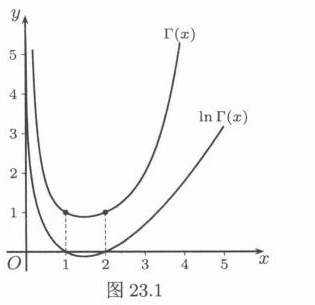
\includegraphics[width=.42\linewidth]{figures/lower/ch23/fig-23-1.png}
\end{center}

\begin{xremark}
1 从积分定义 (23.10) 出发，利用递推公式 (23.12) 可以将 $\Gamma$ 函数的定义域开拓如下。将 (23.12) 变形为
\begin{equation}
  \Gamma(x)=\frac{\Gamma(x+1)}{x}.
  \tag{23.13}
\end{equation}
注意到右边当 $-1<x<0$ 时也有定义，于是我们用 (23.13) 的右边来定义 $-1<x<0$ 时的 $\Gamma$ 函数的值，以此类推，$\Gamma$ 函数的定义域可以开拓到除去 0 和负整数的一切实数。当然这样的开拓结果与 (13.37) 的无穷乘积定义完全一致。
\end{xremark}

\begin{xremark}
2 在所列举的 $\Gamma$ 函数的性质中，前三个在一般教科书中都有。为证明 $\ln\Gamma(x)$ 下凸，从 §8.4 中的下凸函数的定义出发，用无穷限积分的 Hölder 不等式即可得到。最后两个性质的证明比较困难，见下面的 23.3.4 小节。
\end{xremark}

\begin{xremark}
3 在本章末的图 23.2 显示了延拓后的 $\Gamma$ 函数在区间 $[-5,4.1]$ 上的图像。
\end{xremark}

\subsection{例题}

\begin{xexample}[23.3.1]
设平面 $x=0,y=0,z=0$ 与 $x+y+z=1$ 围成四面体 $V$，证明：
\[
  \iiint_V x^{a-1}y^{b-1}z^{c-1}\,\dd x\dd y\dd z
  =\frac{\Gamma(a)\Gamma(b)\Gamma(c)}{(a+b+c)\Gamma(a+b+c)},\qquad a,b,c>0.
\]
\end{xexample}
\begin{xproof}
作以下计算即可：
\[
\begin{aligned}
  I&=\iiint_V x^{a-1}y^{b-1}z^{c-1}\,\dd x\dd y\dd z\\
  &=\int_0^1\dd x\int_0^{1-x}\dd y\int_0^{1-x-y}x^{a-1}y^{b-1}z^{c-1}\,\dd z\\
  &=\frac1c\int_0^1x^{a-1}\,\dd x\int_0^{1-x}y^{b-1}(1-x-y)^c\,\dd y.
\end{aligned}
\]
再令 $y=(1-x)t$，则
\[
\begin{aligned}
  I&=\frac1c\int_0^1x^{a-1}\,\dd x\int_0^1(1-x)^{b-1}t^{b-1}(1-x)^c(1-t)^c(1-x)\,\dd t\\
  &=\frac1c\int_0^1x^{a-1}(1-x)^{b+c}\,\dd x\int_0^1t^{b-1}(1-t)^c\,\dd t\\
  &=\frac1c\mathrm{B}(a,b+c+1)\mathrm{B}(b,c+1)\\
  &=\frac{\Gamma(a)\Gamma(b)\Gamma(c)}{(a+b+c)\Gamma(a+b+c)}.
\end{aligned}
\]
\end{xproof}

\begin{xexample}[23.3.2]
确定 $\alpha,\beta,\gamma$，使
\[
  I=\iiint_D\frac{\dd x\dd y\dd z}{1+x^\alpha+y^\beta+z^\gamma}<+\infty,
\]
并求 $I$ 的值，其中 $D=\{(x,y,z)\mid x\geqslant0,y\geqslant0,z\geqslant0\}$。
\end{xexample}
\begin{xsolution}
首先应该有 $\alpha>0,\beta>0,\gamma>0$。至于进一步的条件，我们将在计算中得到。令 $x=u^{2/\alpha},y=v^{2/\beta},z=w^{2/\gamma}$，则
\[
  I=\frac8{\alpha\beta\gamma}\iiint_\Omega\frac{u^{2/\alpha-1}v^{2/\beta-1}w^{2/\gamma-1}}{1+u^2+v^2+w^2}\,\dd u\dd v\dd w,
\]
其中 $\Omega=\{(u,v,w)\mid u\geqslant0,v\geqslant0,w\geqslant0\}$。再作球坐标变换
\[
  u=\rho\sin\varphi\cos\theta,\quad v=\rho\sin\varphi\sin\theta,\quad w=\rho\cos\varphi,
\]
\[
  \rho\geqslant0,\qquad0\leqslant\varphi\leqslant\frac\pi2,\qquad0\leqslant\theta\leqslant\frac\pi2,
\]
则
\[
\begin{aligned}
I={}&\frac8{\alpha\beta\gamma}\int_0^{\pi/2}\cos^{2/\alpha-1}\theta\sin^{2/\beta-1}\theta\,\dd\theta
\int_0^{\pi/2}\sin^{2(1/\alpha+1/\beta)-1}\varphi\cos^{2/\gamma-1}\varphi\,\dd\varphi\\
&\times\int_0^{+\infty}\frac{\rho^{2(1/\alpha+1/\beta+1/\gamma)-1}}{1+\rho^2}\,\dd\rho\\
={}&\frac1{\alpha\beta\gamma}\mathrm{B}\left(\frac1\alpha,\frac1\beta\right)
\mathrm{B}\left(\frac1\alpha+\frac1\beta,\frac1\gamma\right)
\int_0^{+\infty}\frac{t^{1/\alpha+1/\beta+1/\gamma-1}}{1+t}\,\dd t.
\end{aligned}
\]
可见当且仅当 $\dfrac1\alpha+\dfrac1\beta+\dfrac1\gamma<1$ 时后一个积分收敛，并且有
\[
  \int_0^{+\infty}\frac{t^{1/\alpha+1/\beta+1/\gamma-1}}{1+t}\,\dd t
  =\mathrm{B}\left(\frac1\alpha+\frac1\beta+\frac1\gamma,1-\left(\frac1\alpha+\frac1\beta+\frac1\gamma\right)\right),
\]
这样便得到
\[
  I=\frac1{\alpha\beta\gamma}\Gamma\left(\frac1\alpha\right)\Gamma\left(\frac1\beta\right)\Gamma\left(\frac1\gamma\right)
  \Gamma\left(1-\left(\frac1\alpha+\frac1\beta+\frac1\gamma\right)\right).
\]
\end{xsolution}

\begin{xexample}[23.3.3]
求积分（见上册 395 页练习题 6(2)）
\[
  I(t)=\int_0^{+\infty}\ee^{-(x^2+t^2/x^2)}\,\dd x,\qquad t>0.
\]
\end{xexample}
\begin{xsolution}
\textbf{解 1}\quad 由 M-判别法，$I(t)$ 关于 $t>0$ 是一致收敛的，形式上求导得
\[
  I'(t)=\int_0^{+\infty}\ee^{-(x^2+t^2/x^2)}\left(-\frac{2t}{x^2}\right)\dd x.
\]
$\forall t_0>0$，上述积分在 $t_0$ 的邻域上一致收敛，所以上面的求导可行。令 $x=1/y$，则
\[
  I'(t)=\int_{+\infty}^{0}\ee^{-(1/y^2+y^2t^2)}2t\,\dd y.
\]
再令 $yt=z$，则
\[
  I'(t)=-2\int_0^{+\infty}\ee^{-(z^2+t^2/z^2)}\,\dd z=-2I(t).
\]
所以
\[
  \ln I(t)=-2t+C,\qquad I(t)=C\ee^{-2t}.
\]
考虑到 $I(0)=\displaystyle\int_0^{+\infty}\ee^{-x^2}\,\dd x=\dfrac{\sqrt\pi}{2}$，所以
\[
  I(t)=\frac{\sqrt\pi}{2}\ee^{-2t}.
\]

\textbf{解 2}\quad 下面的方法需要的工具不多，但不容易想到：令 $y=t/x$，则
\[
  I(t)=\int_0^{+\infty}\ee^{-(t^2/y^2+y^2)}\frac{t}{y^2}\,\dd y.
\]
与原表达式相加得
\[
\begin{aligned}
  2I(t)&=\int_0^{+\infty}\ee^{-(x^2+t^2/x^2)}\left(1+\frac{t}{x^2}\right)\dd x\\
  &=\ee^{-2t}\int_0^{+\infty}\ee^{-(x-t/x)^2}\,\dd\left(x-\frac tx\right)\\
  &=\ee^{-2t}\int_{-\infty}^{+\infty}\ee^{-u^2}\,\dd u=\sqrt\pi\ee^{-2t}.
\end{aligned}
\]
\end{xsolution}

\begin{xexample}[23.3.4]
证明 Riemann 的 zeta 函数的积分形式
\[
  \zeta(s)=\sum_{n=1}^{\infty}\frac1{n^s}=\frac1{\Gamma(s)}\int_0^{+\infty}\frac{x^{s-1}}{\ee^x-1}\,\dd x,
  \qquad s>1.
\]
\end{xexample}
\begin{xproof}
对于 $x>0$ 有展开式
\[
  \frac1{\ee^x-1}=\frac{\ee^{-x}}{1-\ee^{-x}}=\ee^{-x}(1+\ee^{-x}+\ee^{-2x}+\cdots)=\sum_{n=1}^{\infty}\ee^{-nx}.
\]
于是 $\forall A>0$ 有
\[
  \int_0^A\frac{x^{s-1}}{\ee^x-1}\,\dd x
  =\int_0^A x^{s-1}\left(\sum_{n=1}^{\infty}\ee^{-nx}\right)\dd x.
\]
对于固定的 $s>1$，级数 $\sum_{n=1}^{\infty}x^{s-1}\ee^{-nx}$ 关于 $x\in[0,+\infty)$ 是一致收敛的，所以
\[
\begin{aligned}
  \int_0^A\frac{x^{s-1}}{\ee^x-1}\,\dd x
  &=\sum_{n=1}^{\infty}\int_0^A x^{s-1}\ee^{-nx}\,\dd x\\
  &=\sum_{n=1}^{\infty}\frac1{n^s}\int_0^{nA}y^{s-1}\ee^{-y}\,\dd y.
\end{aligned}
\]
这个级数对于 $A\in[0,+\infty)$ 是一致收敛的，于是令 $A\to+\infty$，得
\[
  \int_0^{+\infty}\frac{x^{s-1}}{\ee^x-1}\,\dd x=\Gamma(s)\sum_{n=1}^{\infty}\frac1{n^s}.
\]
\end{xproof}

\begin{xexample}[23.3.5]
求 $\displaystyle\int_0^1\frac{\ln x}{1-x}\,\dd x$。
\end{xexample}
\begin{xsolution}
令 $x=\ee^{-t}$，则
\[
  \int_0^1\frac{\ln x}{1-x}\,\dd x=-\int_0^{+\infty}\frac{t}{\ee^t-1}\,\dd t.
\]
在上题的结论中取 $s=2$，则
\[
  \int_0^1\frac{\ln x}{1-x}\,\dd x=-\Gamma(2)\sum_{n=1}^{\infty}\frac1{n^2}=-\frac{\pi^2}{6}.
\]
\end{xsolution}

\begin{xexample}[23.3.6]
求 $I=\displaystyle\iiint_\Omega(\sqrt{a^2-x^2-y^2})^p\,\dd x\dd y\dd z$，其中 $a>0,p\geqslant0,\Omega$ 是球体 $x^2+y^2+z^2\leqslant a^2$ 被圆柱面 $x^2+y^2=ay$ 割下的区域（即 Viviani 体）。
\end{xexample}
\begin{xsolution}
见图 22.11（现在 $x,y$ 轴的位置有变化）。用柱坐标系，则
\[
  \Omega=\{(r,\theta,z)\mid0\leqslant\theta\leqslant\pi,
  0\leqslant r\leqslant a\sin\theta,-\sqrt{a^2-r^2}\leqslant z\leqslant\sqrt{a^2-r^2}\}.
\]
于是
\[
\begin{aligned}
I&=\int_0^\pi\dd\theta\int_0^{a\sin\theta}\dd r
\int_{-\sqrt{a^2-r^2}}^{\sqrt{a^2-r^2}}(\sqrt{a^2-r^2})^p r\,\dd z\\
&=\int_0^\pi\dd\theta\int_0^{a\sin\theta}2r(a^2-r^2)^{(p+1)/2}\,\dd r\\
&=-\int_0^\pi\left.\frac2{p+3}(a^2-r^2)^{(p+3)/2}\right|_0^{a\sin\theta}\dd\theta\\
&=\frac{4a^{p+3}}{p+3}\int_0^{\pi/2}(1-\cos^{p+3}\theta)\,\dd\theta\\
&=\frac{4a^{p+3}}{p+3}\left(\frac\pi2-
\frac{\Gamma\left(\frac{p+4}{2}\right)\Gamma\left(\frac12\right)}{2\Gamma\left(\frac{p+5}{2}\right)}\right).
\end{aligned}
\]
\end{xsolution}

\subsection{\texorpdfstring{$\Gamma$ 函数的特征刻画和几个重要公式的证明}{Gamma 函数的特征刻画和几个重要公式的证明}}

前面已介绍过 $\Gamma$ 函数满足如下三条性质：

1. 当 $x>0$ 时，$\Gamma(x)>0$，且 $\Gamma(1)=1$；

2. $\Gamma(x+1)=x\Gamma(x)$；

3. $\ln\Gamma(x)$ 在 $(0,+\infty)$ 上为下凸函数。

关于 $\Gamma$ 函数的一个非常漂亮的结果是 Bohr（玻尔）与 Mollerup（莫勒鲁普）定理（1922 年），即上面的三条性质完全刻画了 $\Gamma$ 函数。

\begin{xproposition}[23.3.1（Bohr-Mollerup 定理）]
如果定义在 $(0,+\infty)$ 上的函数 $f$ 满足下列三个条件：

(1) $f(x)>0$，且 $f(1)=1$；

(2) $f(x+1)=xf(x)$；

(3) $\ln f(x)$ 是 $(0,+\infty)$ 上的下凸函数，

则 $f(x)\equiv\Gamma(x)$，$x\in(0,+\infty)$。
\end{xproposition}
\begin{xproof}
已知 $\Gamma$ 函数满足上述三条，故只要证明 $f$ 是由 (1)、(2)、(3) 惟一确定的函数就可以了。而由 (2) 只要对 $x\in(0,1)$ 进行证明。令 $\varphi(x)=\ln f(x)$，则
\begin{equation}
  \varphi(x+1)=\varphi(x)+\ln x,\qquad0<x<+\infty.
  \tag{23.14}
\end{equation}
$\varphi(1)=0$，且 $\varphi$ 是下凸函数。设 $0<x<1$，考虑 $\varphi$ 在 $[n,n+1]$、$[n+1,n+1+x]$、$[n+1,n+2]$ 三个闭区间上的差商，有
\begin{equation}
  \ln n=\varphi(n+1)-\varphi(n)\leqslant
  \frac{\varphi(n+1+x)-\varphi(n+1)}{x}
  \leqslant\varphi(n+2)-\varphi(n+1)=\ln(n+1).
  \tag{23.15}
\end{equation}
另一方面，重复 (23.14) 可得
\[
  \varphi(n+1+x)=\varphi(x)+\ln[x(x+1)\cdots(x+n)].
\]
代入 (23.15) 并整理得
\[
  0\leqslant\varphi(x)-\ln\left(\frac{n!n^x}{x(x+1)\cdots(x+n)}\right)
  \leqslant x\ln\left(1+\frac1n\right).
\]
由对数函数的连续性，令 $n\to\infty$，得
\[
  \varphi(x)=\ln\left(\lim_{n\to\infty}\frac{n!n^x}{x(x+1)\cdots(x+n)}\right).
\]
因此
\[
  f(x)=\lim_{n\to\infty}\frac{n!n^x}{x(x+1)\cdots(x+n)}.
\]
利用例题 16.1.4 的结论知 $f(x)=\Gamma(x)$。
\end{xproof}

\begin{xremark}
既然这个定理完全刻画了 $\Gamma$ 函数，因此就可以由它出发导出 $\Gamma$ 函数的基本性质（参见 [7] 的第 7 章），下面就是一个例子。
\end{xremark}

\begin{xproposition}[23.3.2（Legendre 加倍公式）]
对于 $x>0$ 成立
\[
  \Gamma(2x)=\frac{2^{2x-1}}{\sqrt\pi}\Gamma(x)\Gamma\left(x+\frac12\right).
\]
\end{xproposition}
\begin{xproof}
设 $g(x)=\dfrac{2^{x-1}}{\sqrt\pi}\Gamma\left(\dfrac x2\right)\Gamma\left(\dfrac{x+1}{2}\right)$，利用 $\Gamma(\frac12)=\sqrt\pi$，容易检验 $g(x)$ 满足 Bohr-Mollerup 定理中的条件 (1)—(3)，可见
\[
  \Gamma(x)=\frac{2^{x-1}}{\sqrt\pi}\Gamma\left(\frac x2\right)\Gamma\left(\frac{x+1}{2}\right),
\]
将其中 $x$ 换为 $2x$ 就得到所要的加倍公式。
\end{xproof}

\begin{xproposition}[23.3.3（余元公式）]
对于 $0<x<1$ 成立
\[
  \Gamma(x)\Gamma(1-x)=\frac\pi{\sin\pi x}.
\]
\end{xproposition}
根据本节前面的知识，我们可以对余元公式给出下列三种证法：

\textbf{证 1}\quad 利用 $\Gamma$ 函数的 Euler-Gauss 无穷乘积表达式 (23.11)（即 (13.38)）与正弦函数的无穷乘积表达式 (13.30)。具体细节见例题 13.4.4 以及 (13.40)。

\textbf{证 2}\quad 首先利用 $\Gamma$ 函数与 B 函数的关系得到
\[
  \Gamma(x)\Gamma(1-x)=\mathrm{B}(x,1-x)=\int_0^{+\infty}\frac1{y^x(1+y)}\,\dd y,
\]
然后利用例题 16.1.3 的 Euler 积分公式。

\textbf{证 3}\quad 利用上册 402 页参考题 8(2) 的结果：当 $2m+1<2n$ 时，有
\[
  \int_{-\infty}^{+\infty}\frac{x^{2m}}{1+x^{2n}}\,\dd x
  =\frac\pi n\csc\frac{(2m+1)\pi}{2n},
\]
于是有
\[
\begin{aligned}
  \Gamma\left(\frac{2m+1}{2n}\right)\Gamma\left(1-\frac{2m+1}{2n}\right)
  &=\mathrm{B}\left(\frac{2m+1}{2n},1-\frac{2m+1}{2n}\right)\\
  &=\int_0^{+\infty}\frac{y^{(2m+1)/(2n)-1}}{1+y}\,\dd y\\
  &=2n\int_0^{+\infty}\frac{x^{2m}}{1+x^{2n}}\,\dd x\\
  &=\pi\csc\frac{(2m+1)\pi}{2n}.
\end{aligned}
\]
当 $x$ 为无理数时，通过形如 $\dfrac{2m+1}{2n}$ 的有理数取极限。

\begin{xproposition}[23.3.4（$\Gamma$ 函数的 Stirling 公式）]
关于 $\Gamma$ 函数有渐近公式
\begin{equation}
  \Gamma(x+1)\sim\sqrt{2\pi x}\left(\frac x\ee\right)^x\qquad(x\to+\infty).
  \tag{23.16}
\end{equation}
\end{xproposition}
\begin{xproof}
（此证明取自 [46]）在 $\Gamma(x)=\displaystyle\int_0^{+\infty}t^{x-1}\ee^{-t}\,\dd t$ 中令 $t=x(1+u)$，得到
\begin{equation}
  \Gamma(x+1)=x^{x+1}\ee^{-x}\int_{-1}^{+\infty}[(1+u)\ee^{-u}]^x\,\dd u.
  \tag{23.17}
\end{equation}
令
\[
  h(u)=
  \begin{cases}
    \dfrac2{u^2}[u-\ln(1+u)],&-1<u<+\infty,\ u\neq0,\\
    1,&u=0,
  \end{cases}
\]
则 $h$ 在 $(-1,+\infty)$ 上为单调减少的连续函数，并满足
\[
  (1+u)\ee^{-u}=\exp\left(-\frac{u^2}{2}h(u)\right).
\]
于是，对 (23.17) 作代换 $u=s\sqrt{2/x}$，得
\[
  \Gamma(x+1)=x^x\ee^{-x}\sqrt{2x}\int_{-\infty}^{+\infty}\psi_x(s)\,\dd s,
\]
其中
\[
  \psi_x(s)=
  \begin{cases}
    \exp\left[-s^2h\left(s\sqrt{\frac2x}\right)\right],&-\sqrt{\frac x2}<s<+\infty,\\
    0,&s\leqslant-\sqrt{\frac x2}.
  \end{cases}
\]
可以验证：

(1) 对每个 $s$ 而言，当 $x\to+\infty$ 时，$\psi_x(s)\to\ee^{-s^2}$；

(2) 当 $x\geqslant1$ 时，对 $s>0$，有 $0<\psi_x(s)<\psi_1(s)$；

(3) 对 $s<0$，有 $0<\psi_x(s)<\ee^{-s^2}$；

(4) 对任意 $A>0$，含参变量 $x$ 的广义积分 $\displaystyle\int_{-\infty}^{+\infty}\psi_x(s)\,\dd s$ 在闭区间 $[-A,A]$ 上一致收敛；

(5) $\displaystyle\int_0^{+\infty}\psi_1(s)\,\dd s$ 收敛。

因而，就可以得到
\[
  \lim_{x\to+\infty}\int_{-\infty}^{+\infty}\psi_x(s)\,\dd s
  =\int_{-\infty}^{+\infty}\ee^{-s^2}\,\dd s=\sqrt\pi,
\]
即
\[
  \lim_{x\to+\infty}\frac{\Gamma(x+1)}{\sqrt{2\pi x}x^x\ee^{-x}}=1,
\]
这就是关于 $\Gamma$ 函数的 Stirling 公式 (23.16)。
\end{xproof}

\begin{xremark}
这只是关于 $\Gamma$ 函数的 Stirling 公式的最简单形式。与上册 363 页 (11.31) 类似的关于 $\Gamma$ 函数的一般 Stirling 公式见 [18]（第二卷的 540 小节）等参考书。
\end{xremark}

\subsection{练习题}
\begin{xexercise}[1]
计算
  \begin{enumerate}[label=(\arabic*)]
    \item $\displaystyle\int_0^1\frac{\dd x}{\sqrt{x\ln(1/x)}}$；
    \item $\displaystyle\int_0^{+\infty}\frac{\sqrt[4]{x}}{(1+x)^2}\,\dd x$。
  \end{enumerate}
\end{xexercise}
\begin{xsolution}
\textbf{(1)}
\[
I_1=\int_0^1\frac{\dd x}{\sqrt{x\ln(1/x)}}.
\]
令 $t=\ln(1/x)$，即 $x=\ee^{-t}$，则
\[
\begin{aligned}
I_1
&=\int_0^{+\infty}\ee^{-t/2}t^{-1/2}\,\dd t\\
&=\sqrt2\int_0^{+\infty}\ee^{-u}u^{-1/2}\,\dd u
=\sqrt2\,\Gamma\left(\frac12\right).
\end{aligned}
\]
故
\[
\boxed{I_1=\sqrt{2\pi}}.
\]

\textbf{(2)}
\[
I_2=\int_0^{+\infty}\frac{x^{1/4}}{(1+x)^2}\,\dd x.
\]
由 B 函数的无穷区间表示，
\[
I_2=\mathrm{B}\left(\frac54,\frac34\right)
=\Gamma\left(\frac54\right)\Gamma\left(\frac34\right).
\]
再用 $\Gamma(5/4)=\frac14\Gamma(1/4)$ 及余元公式，
\[
\Gamma\left(\frac14\right)\Gamma\left(\frac34\right)
=\frac\pi{\sin(\pi/4)}=\pi\sqrt2.
\]
于是
\[
\boxed{I_2=\frac{\pi\sqrt2}{4}=\frac\pi{2\sqrt2}}.
\]
\end{xsolution}


\begin{xexercise}[2]
试用 $\Gamma$ 函数或 B 函数表示
  \begin{enumerate}[label=(\arabic*)]
    \item $\displaystyle\int_0^{\pi/2}\tan^\alpha x\,\dd x$（$|\alpha|<1$）；
    \item $\displaystyle\int_{-1}^1(1+x)^a(1-x)^b\,\dd x$（$a,b>0$）。
  \end{enumerate}
\end{xexercise}
\begin{xsolution}
\textbf{(1)} 对 $|\alpha|<1$，
\[
\begin{aligned}
\int_0^{\pi/2}\tan^\alpha x\,\dd x
&=\int_0^{\pi/2}\sin^\alpha x\cos^{-\alpha}x\,\dd x\\
&=\frac12\mathrm{B}\left(\frac{\alpha+1}{2},\frac{1-\alpha}{2}\right).
\end{aligned}
\]
两个 B 参数之和为 $1$，由余元公式
\[
\boxed{
\int_0^{\pi/2}\tan^\alpha x\,\dd x
=\frac\pi{2\cos(\pi\alpha/2)},
\qquad |\alpha|<1.}
\]

\textbf{(2)} 令 $x=2t-1$，则
\[
\begin{aligned}
\int_{-1}^1(1+x)^a(1-x)^b\,\dd x
&=2^{a+b+1}\int_0^1t^a(1-t)^b\,\dd t\\
&=2^{a+b+1}\mathrm{B}(a+1,b+1).
\end{aligned}
\]
因此
\[
\boxed{
\int_{-1}^1(1+x)^a(1-x)^b\,\dd x
=2^{a+b+1}\frac{\Gamma(a+1)\Gamma(b+1)}{\Gamma(a+b+2)}.}
\]
\end{xsolution}


\begin{xexercise}[3]
$n$ 为正整数，$p>0$，证明：
  \[
    \mathrm{B}(p,n)=\frac{(n-1)!}{p(p+1)\cdots(p+n-1)}.
  \]
\end{xexercise}
\begin{xsolution}
由 B 函数递推公式
\[
\mathrm{B}(p,q+1)=\frac q{p+q}\mathrm{B}(p,q)
\]
以及
\[
\mathrm{B}(p,1)=\int_0^1x^{p-1}\,\dd x=\frac1p,
\]
反复递推得到
\[
\begin{aligned}
\mathrm{B}(p,n)
&=\frac{n-1}{p+n-1}\frac{n-2}{p+n-2}\cdots
\frac1{p+1}\mathrm{B}(p,1)\\
&=\frac{(n-1)!}{p(p+1)\cdots(p+n-1)}.
\end{aligned}
\]
即得所证。
\end{xsolution}


\begin{xexercise}[4]
证明：$\ln\Gamma(x)$ 是下凸函数。
\end{xexercise}
\begin{xsolution}
任取 $x,y>0$ 与 $0<\lambda<1$。由 $\Gamma$ 函数积分表示，
\[
\begin{aligned}
\Gamma(\lambda x+(1-\lambda)y)
&=\int_0^{+\infty}
t^{\lambda(x-1)+(1-\lambda)(y-1)}\ee^{-t}\,\dd t\\
&=\int_0^{+\infty}
\left(t^{x-1}\ee^{-t}\right)^\lambda
\left(t^{y-1}\ee^{-t}\right)^{1-\lambda}\dd t.
\end{aligned}
\]
对指数 $1/\lambda$ 与 $1/(1-\lambda)$ 应用 Hölder 不等式，得
\[
\Gamma(\lambda x+(1-\lambda)y)
\leqslant \Gamma(x)^\lambda\Gamma(y)^{1-\lambda}.
\]
两边取对数，
\[
\ln\Gamma(\lambda x+(1-\lambda)y)
\leqslant\lambda\ln\Gamma(x)+(1-\lambda)\ln\Gamma(y).
\]
这正是 $\ln\Gamma$ 的下凸性。若 $x\neq y$，Hölder 等号条件不成立，故事实上为严格下凸。
\end{xsolution}


\begin{xexercise}[5]
按照下列步骤证明公式 $\mathrm{B}(p,q)=\dfrac{\Gamma(p)\Gamma(q)}{\Gamma(p+q)}$：
  \begin{enumerate}[label=(\arabic*)]
    \item $\displaystyle\Gamma(p)=2\int_0^{+\infty}u^{2p-1}\ee^{-u^2}\,\dd u$；
    \item $\displaystyle\Gamma(p)\Gamma(q)=\lim_{A\to+\infty}4\iint_{G(A)}f(u,v)\,\dd u\dd v$，其中
    \[
      f(u,v)=u^{2p-1}v^{2q-1}\ee^{-(u^2+v^2)},
    \]
    \[
      G(A)=\{(u,v)\mid0\leqslant u\leqslant A,0\leqslant v\leqslant A\};
    \]
    \item 令 $D(R)=\{(r,\theta)\mid0\leqslant r\leqslant R,0\leqslant\theta\leqslant\frac\pi2\}$，则
    \[
      \lim_{A\to+\infty}\iint_{D(A)}f(u,v)\,\dd u\dd v
      =\frac14\mathrm{B}(p,q)\Gamma(p+q),
    \]
    \[
      \lim_{A\to+\infty}\iint_{D(\sqrt2A)}f(u,v)\,\dd u\dd v
      =\frac14\mathrm{B}(p,q)\Gamma(p+q);
    \]
    \item $\displaystyle\mathrm{B}(p,q)=\frac{\Gamma(p)\Gamma(q)}{\Gamma(p+q)}$。
  \end{enumerate}
\end{xexercise}
\begin{xsolution}
\textbf{(1)} 在 $\Gamma(p)$ 的定义中令 $t=u^2$，则
\[
\Gamma(p)=\int_0^{+\infty}t^{p-1}\ee^{-t}\,\dd t
=2\int_0^{+\infty}u^{2p-1}\ee^{-u^2}\,\dd u.
\]

\textbf{(2)} 因被积函数非负，由 Tonelli 定理及单调收敛，
\[
\begin{aligned}
\Gamma(p)\Gamma(q)
&=4\int_0^{+\infty}\int_0^{+\infty}
 u^{2p-1}v^{2q-1}\ee^{-(u^2+v^2)}\,\dd u\dd v\\
&=\lim_{A\to+\infty}4\iint_{G(A)}f(u,v)\,\dd u\dd v.
\end{aligned}
\]

\textbf{(3)} 在第一象限极坐标中，$u=r\cos\theta,v=r\sin\theta$。因此
\[
\begin{aligned}
\iint_{D(R)}f(u,v)\,\dd u\dd v
&=\int_0^{\pi/2}\cos^{2p-1}\theta\sin^{2q-1}\theta\,\dd\theta\\
&\quad\times\int_0^R r^{2p+2q-1}\ee^{-r^2}\,\dd r\\
&=\frac14\mathrm{B}(p,q)
\int_0^{R^2}s^{p+q-1}\ee^{-s}\,\dd s.
\end{aligned}
\]
令 $R\to+\infty$，得到
\[
\lim_{R\to+\infty}\iint_{D(R)}f
=\frac14\mathrm{B}(p,q)\Gamma(p+q).
\]
特别地，取 $R=A$ 或 $R=\sqrt2A$ 都得到题中两式。

\textbf{(4)} 几何上有
\[
D(A)\subset G(A)\subset D(\sqrt2A).
\]
又 $f\geqslant0$，所以
\[
\iint_{D(A)}f\leqslant\iint_{G(A)}f
\leqslant\iint_{D(\sqrt2A)}f.
\]
令 $A\to+\infty$，左右两端均趋于
$\frac14\mathrm{B}(p,q)\Gamma(p+q)$。由夹逼定理，
\[
\lim_{A\to+\infty}4\iint_{G(A)}f
=\mathrm{B}(p,q)\Gamma(p+q).
\]
结合第 (2) 步，
\[
\Gamma(p)\Gamma(q)=\mathrm{B}(p,q)\Gamma(p+q),
\]
故
\[
\boxed{\mathrm{B}(p,q)=\frac{\Gamma(p)\Gamma(q)}{\Gamma(p+q)}}.
\]
\end{xsolution}


\section{对于教学的建议}

\subsection{学习要点}

1. 含参变量积分是我们遇到的又一种新的函数表示方式。对于它的分析性质的研究，如连续性、可微性和可积性等，涉及积分运算和其他分析运算的运算次序的交换性。一致收敛性给出了保证交换运算次序的重要条件。在很多情况下，可以用 M-判别法判断一致收敛性，这是应该熟练掌握的。

2. 用嵌入法计算广义积分的值体现了数学中的“嵌入”思想。假设要考虑一个 1 维的问题（比如计算一个定积分）。我们不妨把这个问题放到更高维的框架中，例如再引入一个参变量，把这个积分作为含参变量积分的特例。由于在引入的高维框架中，我们可以有更多的可施展数学工具（如积分、微分等）的天地，就有可能从另一个角度（而这一个角度是我们引入高维框架后带来的）把我们的问题简化，从而达到解决原有问题的目的。在具体计算过程中，要作一些分析，在什么地方引入参变量比较合适，用微分法还是用积分法，都是有讲究的。比如计算 Dirichlet 积分 $\displaystyle\int_0^{+\infty}\frac{\sin x}{x}\,\dd x$。把它看成是含参变量积分 $\varphi(\alpha)=\displaystyle\int_0^{+\infty}\ee^{-\alpha x}\frac{\sin x}{x}\,\dd x$ 当 $\alpha=0$ 时的值。引入因子 $\ee^{-\alpha x}$ 有两个作用，对 $\alpha$ 求导可消去导致不可积的因子 $1/x$，同时 $\ee^{-\alpha x}$ 又是收敛因子，保证了在 $\alpha>0$ 时积分 $\displaystyle\int_0^{+\infty}\left(\ee^{-\alpha x}\frac{\sin x}{x}\right)'_\alpha\dd x$ 的内闭一致收敛性。故可在积分号下求导，则有
\[
  \varphi'(\alpha)=-\int_0^{+\infty}\ee^{-\alpha x}\sin x\,\dd x=-\frac1{1+\alpha^2}.
\]
再积分就有 $\varphi(\alpha)=\dfrac\pi2-\arctan\alpha,\alpha>0$。如果 $\varphi(\alpha)$ 在 $[0,+\infty)$ 上连续，则
\[
  \int_0^{+\infty}\frac{\sin x}{x}\,\dd x=\varphi(0)=\lim_{\alpha\to0^+}\varphi(\alpha)=\frac\pi2.
\]

3. 含参变量积分的一致收敛性的判别与函数项级数有许多类似之处，同时也要注意到利用积分自身的特点，如变量代换、分部积分等。以 $\displaystyle\int_1^{+\infty}\frac{\cos x^2}{x^p}\,\dd x$ 为例，作变换 $x^2=t$，就化为 $\displaystyle\int_1^{+\infty}\frac{\cos t}{2t^{(p+1)/2}}\,\dd t$，成为我们熟悉的类型。

4. B 函数的三个积分表达式，各有各的长处，应加以记忆。这样，遇到相应的积分，就可写成特殊的 B 值，再利用余元公式等得到积分值。

5. \textbf{对习题课的建议}\quad 许多学生对讨论含参变量广义积分的一致收敛性有畏难情绪，习题课上要由浅入深地进行引导，分析难点，找出办法。大多数题目只需使用 M-判别法。在用嵌入法计算一些特殊的广义积分的值时，如果觉得证明计算合理性（如检验一致收敛性等）的过程较长，可以在解题时先进行形式运算，算出积分值后再给出运算合理性的证明。

本章的内容综合性强，计算题大多具有一定的技巧性。因此应在习题课上作比较系统的示范和总结。

\subsection{参考题}
\begin{xreferenceproblem}[1]
设 $f(x,t),f_x(x,t)$ 连续，记
  \[
    u(x,t)=\frac1{2a}\int_0^t\dd\tau\int_{x-a(t-\tau)}^{x+a(t-\tau)}f(\xi,\tau)\,\dd\xi,
  \]
  其中 $a$ 为正常数，证明：$u(x,t)$ 满足
  \[
    \frac{\partial^2u}{\partial t^2}=a^2\frac{\partial^2u}{\partial x^2}+f(x,t).
  \]
\end{xreferenceproblem}
\begin{xsolution}
记
\[
A=x-a(t-\tau),\qquad B=x+a(t-\tau).
\]
由 Leibniz 公式，注意当 $\tau=t$ 时 $A=B=x$，有
\[
\begin{aligned}
u_t(x,t)
&=\frac12\int_0^t[f(B,\tau)+f(A,\tau)]\,\dd\tau.
\end{aligned}
\]
再对 $t$ 求导，
\[
\begin{aligned}
u_{tt}(x,t)
&=f(x,t)+\frac a2\int_0^t
[f_x(B,\tau)-f_x(A,\tau)]\,\dd\tau.
\end{aligned}
\]
另一方面，对 $x$ 求导，
\[
u_x(x,t)=\frac1{2a}\int_0^t[f(B,\tau)-f(A,\tau)]\,\dd\tau,
\]
故
\[
u_{xx}(x,t)=\frac1{2a}\int_0^t
[f_x(B,\tau)-f_x(A,\tau)]\,\dd\tau.
\]
于是
\[
u_{tt}(x,t)=f(x,t)+a^2u_{xx}(x,t),
\]
即得所证。
\end{xsolution}


\begin{xreferenceproblem}[2]
设 $n$ 为正整数，证明 Bessel 函数
  \[
    J_n(x)=\frac1\pi\int_0^\pi\cos(n\varphi-x\sin\varphi)\,\dd\varphi
  \]
  满足
  \[
    x^2J_n''(x)+xJ_n'(x)+(x^2-n^2)J_n(x)=0.
  \]
\end{xreferenceproblem}
\begin{xsolution}
令
\[
\Theta=n\varphi-x\sin\varphi.
\]
因积分区间有限，可逐次在积分号下求导：
\[
J_n'(x)=\frac1\pi\int_0^\pi\sin\Theta\sin\varphi\,\dd\varphi,
\]
\[
J_n''(x)=-\frac1\pi\int_0^\pi\cos\Theta\sin^2\varphi\,\dd\varphi.
\]
于是
\[
\begin{aligned}
&\pi[x^2J_n''+xJ_n'+(x^2-n^2)J_n]\\
&=\int_0^\pi
\left[(x^2\cos^2\varphi-n^2)\cos\Theta
+x\sin\varphi\sin\Theta\right]\dd\varphi.
\end{aligned}
\]
而
\[
\begin{aligned}
\frac{\dd}{\dd\varphi}[(n+x\cos\varphi)\sin\Theta]
&=(n^2-x^2\cos^2\varphi)\cos\Theta
-x\sin\varphi\sin\Theta.
\end{aligned}
\]
故上面的被积函数恰为该导数的负值。因此
\[
\begin{aligned}
\pi[x^2J_n''+xJ_n'+(x^2-n^2)J_n]
&=-[(n+x\cos\varphi)\sin\Theta]_0^\pi=0,
\end{aligned}
\]
因为 $\sin\Theta=0$ 在 $\varphi=0,\pi$ 均成立。所证方程成立。
\end{xsolution}


\begin{xreferenceproblem}[3]
设 $f(x)$ 在 $[0,1]$ 上连续可微，且 $f(0)=0$，定义
  \[
    \varphi(x)=\int_0^x\frac{f(t)}{\sqrt{x-t}}\,\dd t,\quad0<x\leqslant1,\quad\varphi(0)=0.
  \]
  证明：
  \begin{enumerate}[label=(\arabic*)]
    \item $\varphi(x)$ 在 $[0,1]$ 上一阶连续可导，且
    \[
      \varphi'(x)=\int_0^x\frac{f'(t)}{\sqrt{x-t}}\,\dd t,\quad0<x\leqslant1,\quad\varphi'(0)=0;
    \]
    \item $\displaystyle f(x)=\frac1\pi\int_0^x\frac{\varphi'(t)}{\sqrt{x-t}}\,\dd t$，$0<x\leqslant1$。
  \end{enumerate}
\end{xreferenceproblem}
\begin{xsolution}
\textbf{(1)} 由 $f(0)=0$，
\[
f(t)=\int_0^t f'(s)\,\dd s.
\]
代入并交换有限区域上的积分次序：
\[
\begin{aligned}
\varphi(x)
&=\int_0^x\frac{\dd t}{\sqrt{x-t}}
\int_0^t f'(s)\,\dd s\\
&=\int_0^x f'(s)\,\dd s
\int_s^x\frac{\dd t}{\sqrt{x-t}}\\
&=2\int_0^x f'(s)\sqrt{x-s}\,\dd s.
\end{aligned}
\]
故对 $x>0$，
\[
\boxed{
\varphi'(x)=\int_0^x\frac{f'(s)}{\sqrt{x-s}}\,\dd s.}
\]
若 $M=\max_{[0,1]}|f'|$，则由
\[
\varphi(x)=2\int_0^x f'(s)\sqrt{x-s}\,\dd s
\]
可得
\[
\left|\frac{\varphi(x)-\varphi(0)}x\right|
\leqslant\frac{2M}{x}\int_0^x\sqrt{x-s}\,\dd s
=\frac{4M}{3}\sqrt x\to0.
\]
故 $\varphi$ 在 $0$ 处可导，且 $\varphi'(0)=0$。另一方面，对 $x>0$，
\[
|\varphi'(x)|\leqslant2M\sqrt x\to0,
\]
所以 $\varphi'$ 在 $0$ 处连续。对 $x_0>0$，把上式令 $s=xu$ 可写成
\[
\varphi'(x)=\sqrt x\int_0^1\frac{f'(xu)}{\sqrt{1-u}}\,\dd u.
\]
由 $f'$ 在 $[0,1]$ 上一致连续，且 $(1-u)^{-1/2}$ 在 $(0,1)$ 上可积，右端关于 $x$ 连续。因此 $\varphi\in C^1[0,1]$。

\textbf{(2)} 将上式代入题中右端，
\[
\begin{aligned}
\int_0^x\frac{\varphi'(t)}{\sqrt{x-t}}\,\dd t
&=\int_0^x\frac{\dd t}{\sqrt{x-t}}
\int_0^t\frac{f'(s)}{\sqrt{t-s}}\,\dd s\\
&=\int_0^x f'(s)\,\dd s
\int_s^x\frac{\dd t}{\sqrt{(t-s)(x-t)}}.
\end{aligned}
\]
内层令 $t=s+(x-s)u$，得到
\[
\int_s^x\frac{\dd t}{\sqrt{(t-s)(x-t)}}
=\int_0^1\frac{\dd u}{\sqrt{u(1-u)}}=\pi.
\]
故
\[
\int_0^x\frac{\varphi'(t)}{\sqrt{x-t}}\,\dd t
=\pi\int_0^x f'(s)\,\dd s=\pi f(x),
\]
即
\[
\boxed{
f(x)=\frac1\pi\int_0^x\frac{\varphi'(t)}{\sqrt{x-t}}\,\dd t.}
\]
\end{xsolution}


\begin{xreferenceproblem}[4]
设 $f(x)$ 在 $[0,A]$ 上单调（$A>0$），证明：
  \[
    \lim_{\alpha\to+\infty}\int_0^A f(x)\frac{\sin\alpha x}{x}\,\dd x=\frac\pi2f(0^+).
  \]
\end{xreferenceproblem}
\begin{xsolution}
记 $L=f(0^+)$，并令 $g(x)=f(x)-L$。则 $g$ 单调且 $g(0^+)=0$。分解
\[
\int_0^A f(x)\frac{\sin\alpha x}{x}\,\dd x
=L\int_0^A\frac{\sin\alpha x}{x}\,\dd x
+\int_0^A g(x)\frac{\sin\alpha x}{x}\,\dd x.
\]
第一项令 $u=\alpha x$ 后，由 Dirichlet 积分得
\[
\int_0^A\frac{\sin\alpha x}{x}\,\dd x
=\int_0^{\alpha A}\frac{\sin u}{u}\,\dd u\to\frac\pi2.
\]
只需证明第二项趋于 $0$。

任给 $\varepsilon>0$，由 $g(0^+)=0$ 可取 $0<\delta<A$，使
$|g(x)|<\varepsilon$ 对 $0<x<\delta$ 成立。记
\[
S_\alpha(x)=\int_0^x\frac{\sin\alpha t}{t}\,\dd t.
\]
Dirichlet 积分的部分积分一致有界，即存在常数 $C$ 使
$|S_\alpha(x)|\leqslant C$ 对所有 $\alpha,x>0$ 成立。由于 $g$ 单调，在 $[0,\delta]$ 上作 Riemann--Stieltjes 分部积分可得
\[
\left|\int_0^\delta g(x)\frac{\sin\alpha x}{x}\,\dd x\right|
\leqslant2C|g(\delta)|\leqslant2C\varepsilon.
\]
在 $[\delta,A]$ 上，$g(x)/x$ 为有界可积函数，由 Riemann--Lebesgue 引理
\[
\int_\delta^A\frac{g(x)}x\sin\alpha x\,\dd x\to0.
\]
先令 $\alpha\to\infty$，再令 $\varepsilon\to0$，便得第二项趋于 $0$。于是
\[
\boxed{
\lim_{\alpha\to+\infty}
\int_0^A f(x)\frac{\sin\alpha x}{x}\,\dd x
=\frac\pi2f(0^+).}
\]
\end{xsolution}


\begin{xreferenceproblem}[5]
设 $F(t)=t\displaystyle\int_0^{+\infty}\ee^{-tx}f(x)\,\dd x$，其中 $f(x)$ 在 $[0,b]$ 上有界可积（$\forall b>0$），且 $\displaystyle\lim_{x\to+\infty}f(x)=\alpha$，证明：$\displaystyle\lim_{t\to0^+}F(t)=\alpha$。
\end{xreferenceproblem}
\begin{xsolution}
由于 $f(x)\to\alpha$，$f$ 在充分大的半轴上有界；再结合它在有限闭区间上有界，知存在 $M$ 使
\[
|f(x)|\leqslant M\qquad(x\geqslant0).
\]
令 $u=tx$，则
\[
F(t)=\int_0^{+\infty}\ee^{-u}f(u/t)\,\dd u.
\]
对每个固定 $u>0$，当 $t\to0^+$ 时 $u/t\to+\infty$，故
$f(u/t)\to\alpha$。并且
\[
|\ee^{-u}f(u/t)|\leqslant M\ee^{-u},
\]
右端可积。由控制收敛定理，
\[
\boxed{
\lim_{t\to0^+}F(t)
=\alpha\int_0^{+\infty}\ee^{-u}\,\dd u=\alpha.}
\]
\end{xsolution}


\begin{xreferenceproblem}[6]
设 $f(x)$ 连续，且 $\displaystyle\int_{-\infty}^{+\infty}f^2(x)\,\dd x$ 收敛，证明：
  \begin{enumerate}[label=(\arabic*)]
    \item $q(t)=\displaystyle\int_{-\infty}^{+\infty}f(t+u)f(u)\,\dd u$ 在 $(-\infty,+\infty)$ 上连续且有界；
    \item $\displaystyle\lim_{\varepsilon\to0^+}\frac1{2\sqrt{\varepsilon\pi}}\int_{-\infty}^{+\infty}\ee^{-t^2/(4\varepsilon)}g(t)\,\dd t=\int_{-\infty}^{+\infty}f^2(x)\,\dd x$。
  \end{enumerate}
\end{xreferenceproblem}
\begin{xsolution}
\textbf{(1)} 记
\[
q(t)=\int_{-\infty}^{+\infty}f(t+u)f(u)\,\dd u.
\]
由 Cauchy--Schwarz 不等式及平移不改变 $L^2$ 范数，
\[
|q(t)|\leqslant
\left(\int_{-\infty}^{+\infty}f^2(t+u)\,\dd u\right)^{1/2}
\left(\int_{-\infty}^{+\infty}f^2(u)\,\dd u\right)^{1/2}
=\|f\|_2^2.
\]
故 $q$ 有界。

又
\[
|q(t+h)-q(t)|
\leqslant\|f\|_2\,
\|f(\cdot+t+h)-f(\cdot+t)\|_2.
\]
只需用到 $L^2$ 中平移的连续性。这里可直接证明：先取 $R$ 使
$\int_{|x|>R}f^2(x)\,\dd x$ 足够小；在紧区间 $[-R-1,R+1]$ 上 $f$ 一致连续，所以当 $h$ 足够小时，中央部分的平方积分足够小；两端由所选尾积分控制。因此
\[
\|f(\cdot+h)-f\|_2\to0.
\]
所以 $q$ 在 $\RR$ 上连续。

% SOURCE-ERR: 题面第二问的 g(t) 未定义；按第一问定义及右端结论应为 q(t)。
\textbf{(2)} 记
\[
K_\varepsilon(t)=\frac1{2\sqrt{\varepsilon\pi}}
\ee^{-t^2/(4\varepsilon)}.
\]
则 $K_\varepsilon\geqslant0$ 且
\[
\int_{-\infty}^{+\infty}K_\varepsilon(t)\,\dd t=1.
\]
由第一问，$q$ 连续有界，且
\[
q(0)=\int_{-\infty}^{+\infty}f^2(x)\,\dd x.
\]
任给 $\eta>0$，由 $q$ 在 $0$ 连续，取 $\delta>0$ 使
$|q(t)-q(0)|<\eta$ 当 $|t|<\delta$。于是
\[
\begin{aligned}
\left|\int K_\varepsilon(t)q(t)\,\dd t-q(0)\right|
&\leqslant\eta
+2\|q\|_\infty\int_{|t|\geqslant\delta}K_\varepsilon(t)\,\dd t.
\end{aligned}
\]
当 $\varepsilon\to0^+$ 时，Gaussian 尾积分趋于 $0$。再令 $\eta\to0$，得到
\[
\boxed{
\lim_{\varepsilon\to0^+}\frac1{2\sqrt{\varepsilon\pi}}
\int_{-\infty}^{+\infty}\ee^{-t^2/(4\varepsilon)}q(t)\,\dd t
=\int_{-\infty}^{+\infty}f^2(x)\,\dd x.}
\]
\end{xsolution}


\begin{xreferenceproblem}[7]
讨论下列函数在 $(0,1)$ 上的连续性：
  \begin{enumerate}[label=(\arabic*)]
    \item $f(\alpha)=\displaystyle\int_0^{+\infty}\frac{\ee^{-t}}{|\sin t|^\alpha}\,\dd t$；
    \item $g(\alpha)=\displaystyle\int_0^1\frac{f(t)}{\sqrt{|t-\alpha|}}\,\dd t$，其中 $f(t)$ 是 $[0,1]$ 上的有界可积函数。
  \end{enumerate}
\end{xreferenceproblem}
\begin{xsolution}
\textbf{(1)}
\[
F(\alpha)=\int_0^{+\infty}\frac{\ee^{-t}}{|\sin t|^\alpha}\,\dd t,
\qquad0<\alpha<1.
\]
任取 $\alpha_0\in(0,1)$，选 $\beta$ 使 $\alpha_0<\beta<1$，并把参数限制在 $0<\alpha\leqslant\beta$ 的一个邻域。由于 $|\sin t|\leqslant1$，
\[
\frac{\ee^{-t}}{|\sin t|^\alpha}
\leqslant\frac{\ee^{-t}}{|\sin t|^\beta}.
\]
右端在每个 $k\pi$ 附近只有 $|t-k\pi|^{-\beta}$ 型可积奇性。更具体地，在长度为 $\pi$ 的相邻区间上
\[
\int\frac{\dd t}{|\sin t|^\beta}=C_\beta<+\infty
\]
与 $k$ 无关，而因子 $\ee^{-t}$ 使这些区间的贡献按 $\ee^{-k\pi}$ 几何衰减。因此右端在 $(0,+\infty)$ 可积。被积函数对 $\alpha$ 点态连续，故由控制收敛定理，$F$ 在每个 $\alpha_0\in(0,1)$ 连续。

\textbf{(2)}
\[
G(\alpha)=\int_0^1\frac{f(t)}{\sqrt{|t-\alpha|}}\,\dd t,
\qquad0<\alpha<1,
\]
其中 $f$ 有界可积。设 $|f(t)|\leqslant M$。只需证明核
\[
k_\alpha(t)=|t-\alpha|^{-1/2}
\]
在 $L^1(0,1)$ 中关于 $\alpha$ 连续。固定 $\alpha_0\in(0,1)$，令 $h=|\alpha-\alpha_0|$ 足够小。把积分分成
$|t-\alpha_0|<2h$ 与其补集。前一部分中两个核的积分均为 $\bigO(\sqrt h)$。在补集上利用中值定理，
\[
|k_\alpha(t)-k_{\alpha_0}(t)|
\leqslant C h|t-\alpha_0|^{-3/2},
\]
从而
\[
\int_{|t-\alpha_0|\geqslant2h}
|k_\alpha-k_{\alpha_0}|\,\dd t
\leqslant Ch\int_{2h}^1s^{-3/2}\,\dd s
=\bigO(\sqrt h).
\]
故
\[
\|k_\alpha-k_{\alpha_0}\|_1\to0.
\]
于是
\[
|G(\alpha)-G(\alpha_0)|
\leqslant M\|k_\alpha-k_{\alpha_0}\|_1\to0.
\]
所以 $G$ 在 $(0,1)$ 上连续。
\end{xsolution}


\begin{xreferenceproblem}[8]
求曲面 $(x^2+y^2)^2+z^4=y$ 所围立体的体积。
\end{xreferenceproblem}
\begin{xsolution}
用柱坐标
\[
x=r\cos\theta,\qquad y=r\sin\theta.
\]
立体内部满足
\[
r^4+z^4\leqslant r\sin\theta.
\]
因此必须 $0\leqslant\theta\leqslant\pi$，且
\[
0\leqslant r\leqslant(\sin\theta)^{1/3},
\qquad
|z|\leqslant[r(\sin\theta-r^3)]^{1/4}.
\]
故体积为
\[
\begin{aligned}
V
&=2\int_0^\pi\dd\theta
\int_0^{(\sin\theta)^{1/3}}
r[r(\sin\theta-r^3)]^{1/4}\,\dd r\\
&=2\int_0^\pi\dd\theta
\int_0^{(\sin\theta)^{1/3}}
r^{5/4}(\sin\theta-r^3)^{1/4}\,\dd r.
\end{aligned}
\]
对固定 $\theta$ 令
\[
u=\frac{r^3}{\sin\theta}.
\]
则
\[
\int_0^{(\sin\theta)^{1/3}}
r^{5/4}(\sin\theta-r^3)^{1/4}\,\dd r
=\frac13\sin\theta\,
\mathrm{B}\left(\frac34,\frac54\right).
\]
于是
\[
V=\frac23\mathrm{B}\left(\frac34,\frac54\right)
\int_0^\pi\sin\theta\,\dd\theta
=\frac43\mathrm{B}\left(\frac34,\frac54\right).
\]
利用余元公式，
\[
\mathrm{B}\left(\frac34,\frac54\right)
=\Gamma\left(\frac34\right)\Gamma\left(\frac54\right)
=\frac14\Gamma\left(\frac34\right)\Gamma\left(\frac14\right)
=\frac{\pi\sqrt2}{4}.
\]
所以
\[
\boxed{V=\frac{\pi\sqrt2}{3}}.
\]
\end{xsolution}


\begin{xreferenceproblem}[9]
求立体
  \[
    \left(\frac xa\right)^{1/n}+\left(\frac yb\right)^{1/n}+\left(\frac zc\right)^{1/n}\leqslant1,
    \qquad x,y,z\geqslant0
  \]
  的质心的 $x$ 坐标。
\end{xreferenceproblem}
\begin{xsolution}
令
\[
x=au^n,\qquad y=bv^n,\qquad z=cw^n,
\]
则 $u,v,w\geqslant0$ 且 $u+v+w\leqslant1$，Jacobi 行列式为
\[
abc\,n^3u^{n-1}v^{n-1}w^{n-1}.
\]
记标准三维单纯形为 $\Delta$。体积
\[
V=abc\,n^3\iiint_\Delta
u^{n-1}v^{n-1}w^{n-1}\,\dd u\dd v\dd w.
\]
利用 Dirichlet 积分公式
\[
\iiint_\Delta
u^{\alpha-1}v^{\beta-1}w^{\gamma-1}\,\dd u\dd v\dd w
=\frac{\Gamma(\alpha)\Gamma(\beta)\Gamma(\gamma)}
{\Gamma(\alpha+\beta+\gamma+1)},
\]
得到
\[
V=abc\,n^3\frac{\Gamma(n)^3}{\Gamma(3n+1)}.
\]
关于 $yz$ 平面的静矩为
\[
\begin{aligned}
M_{yz}
&=a^2bc\,n^3\iiint_\Delta
u^{2n-1}v^{n-1}w^{n-1}\,\dd u\dd v\dd w\\
&=a^2bc\,n^3
\frac{\Gamma(2n)\Gamma(n)^2}{\Gamma(4n+1)}.
\end{aligned}
\]
因此
\[
\boxed{
\bar x=\frac{M_{yz}}V
=a\frac{\Gamma(2n)\Gamma(3n+1)}
{\Gamma(n)\Gamma(4n+1)}.}
\]
若 $n$ 为正整数，也可写成
\[
\boxed{
\bar x
=a\frac{(2n-1)!(3n)!}{(n-1)!(4n)!}.}
\]
\end{xsolution}


\begin{xreferenceproblem}[10]
求星形线 $x^{2/3}+y^{2/3}=R^{2/3}$ 所包围的面积对 $x$ 轴的惯性矩。
\end{xreferenceproblem}
\begin{xsolution}
由对称性，在 $y\geqslant0$ 时
\[
x_{\max}(y)=\left(R^{2/3}-y^{2/3}\right)^{3/2},
\qquad0\leqslant y\leqslant R.
\]
故
\[
I_x=4\int_0^R y^2
\left(R^{2/3}-y^{2/3}\right)^{3/2}\,\dd y.
\]
令 $y=Rt^{3/2}$，则
\[
\begin{aligned}
I_x
&=6R^4\int_0^1t^{7/2}(1-t)^{3/2}\,\dd t\\
&=6R^4\mathrm{B}\left(\frac92,\frac52\right).
\end{aligned}
\]
而
\[
\mathrm{B}\left(\frac92,\frac52\right)
=\frac{\Gamma(9/2)\Gamma(5/2)}{\Gamma(7)}
=\frac{7\pi}{1024}.
\]
因此
\[
\boxed{I_x=\frac{21\pi}{512}R^4}.
\]
\end{xsolution}


\begin{xreferenceproblem}[11]
设 $f(x)$ 在 $[0,1]$ 中连续，证明：
  \[
    \lim_{t\to+\infty}\int_0^1t\ee^{-t^2x^2}f(x)\,\dd x=\frac{\sqrt\pi}{2}f(0).
  \]
\end{xreferenceproblem}
\begin{xsolution}
令 $u=tx$，则
\[
\int_0^1t\ee^{-t^2x^2}f(x)\,\dd x
=\int_0^t\ee^{-u^2}f(u/t)\,\dd u.
\]
把右端写成
\[
\int_0^{+\infty}\ee^{-u^2}f(u/t)\mathbf{1}_{[0,t]}(u)\,\dd u.
\]
因 $f$ 在 $[0,1]$ 上有界，设 $|f|\leqslant M$，则绝对值不超过
$M\ee^{-u^2}$。对每个固定 $u\geqslant0$，当 $t\to\infty$ 时
$u/t\to0$ 且最终 $u<t$，故被积函数趋于 $\ee^{-u^2}f(0)$。由控制收敛定理，
\[
\boxed{
\lim_{t\to+\infty}
\int_0^1t\ee^{-t^2x^2}f(x)\,\dd x
=f(0)\int_0^{+\infty}\ee^{-u^2}\,\dd u
=\frac{\sqrt\pi}{2}f(0).}
\]
\end{xsolution}


\begin{xreferenceproblem}[12]
设 $\displaystyle\int_0^{+\infty}f(x)\,\dd x$ 收敛，证明：
  \[
    \lim_{y\to0^+}\int_0^{+\infty}\ee^{-xy}f(x)\,\dd x=\int_0^{+\infty}f(x)\,\dd x.
  \]
\end{xreferenceproblem}
\begin{xsolution}
令
\[
F(X)=\int_0^X f(x)\,\dd x,
\qquad
L=\int_0^{+\infty}f(x)\,\dd x.
\]
由假设 $F(X)\to L$，故 $F$ 有界。对 $y>0$，分部积分得
\[
\begin{aligned}
\int_0^{+\infty}\ee^{-xy}f(x)\,\dd x
&=[\ee^{-xy}F(x)]_0^{+\infty}
+y\int_0^{+\infty}\ee^{-xy}F(x)\,\dd x\\
&=y\int_0^{+\infty}\ee^{-xy}F(x)\,\dd x.
\end{aligned}
\]
令 $u=xy$，得到
\[
\int_0^{+\infty}\ee^{-xy}f(x)\,\dd x
=\int_0^{+\infty}\ee^{-u}F(u/y)\,\dd u.
\]
对每个 $u>0$，$y\to0^+$ 时 $F(u/y)\to L$，且 $F$ 有界，所以由控制收敛定理
\[
\lim_{y\to0^+}\int_0^{+\infty}\ee^{-xy}f(x)\,\dd x
=L\int_0^{+\infty}\ee^{-u}\,\dd u=L.
\]
即得所证。
\end{xsolution}


\begin{xreferenceproblem}[13]
求 $\displaystyle\int_0^{+\infty}\cos x^p\,\dd x$，其中 $p>1$。
\end{xreferenceproblem}
\begin{xsolution}
令 $t=x^p$，并记 $s=1/p\in(0,1)$，则
\[
I=\frac1p\int_0^{+\infty}t^{s-1}\cos t\,\dd t.
\]
由 $\Gamma$ 函数的定义，对 $t>0$ 有
\[
\int_0^{+\infty}u^{-s}\ee^{-ut}\,\dd u
=\Gamma(1-s)t^{s-1},
\]
即
\[
t^{s-1}=\frac1{\Gamma(1-s)}
\int_0^{+\infty}u^{-s}\ee^{-ut}\,\dd u.
\]
对任意 $R>0$，由于
\[
\int_0^R\dd t\int_0^{+\infty}u^{-s}\ee^{-ut}\,\dd u
=\Gamma(1-s)\int_0^R t^{s-1}\,\dd t<+\infty,
\]
可以交换积分次序，得到
\[
\int_0^R t^{s-1}\cos t\,\dd t
=\frac1{\Gamma(1-s)}
\int_0^{+\infty}u^{-s}
\left(\int_0^R\ee^{-ut}\cos t\,\dd t\right)\dd u.
\]
而
\[
\int_0^R\ee^{-ut}\cos t\,\dd t
=\frac{u+\ee^{-uR}(-u\cos R+\sin R)}{1+u^2},
\]
故其绝对值不超过
\[
\frac{2u+1}{1+u^2}.
\]
因为 $0<s<1$，函数
\[
u^{-s}\frac{2u+1}{1+u^2}
\]
在 $(0,+\infty)$ 上可积，所以可令 $R\to+\infty$，得到
\[
\int_0^{+\infty}t^{s-1}\cos t\,\dd t
=\frac1{\Gamma(1-s)}
\int_0^{+\infty}\frac{u^{1-s}}{1+u^2}\,\dd u.
\]
令 $u=\tan\theta$，则
\[
\begin{aligned}
\int_0^{+\infty}\frac{u^{1-s}}{1+u^2}\,\dd u
&=\int_0^{\pi/2}\tan^{1-s}\theta\,\dd\theta\\
&=\frac12\mathrm{B}\left(\frac s2,1-\frac s2\right)
=\frac{\pi}{2\sin(\pi s/2)}.
\end{aligned}
\]
再由余元公式
\[
\Gamma(s)\Gamma(1-s)=\frac\pi{\sin\pi s}
\]
以及 $\sin\pi s=2\sin(\pi s/2)\cos(\pi s/2)$，可得
\[
\int_0^{+\infty}t^{s-1}\cos t\,\dd t
=\Gamma(s)\cos\frac{\pi s}{2}.
\]
因此
\[
\boxed{
\int_0^{+\infty}\cos x^p\,\dd x
=\frac1p\Gamma\left(\frac1p\right)
\cos\frac\pi{2p}
=\Gamma\left(1+\frac1p\right)\cos\frac\pi{2p}.}
\]
\end{xsolution}


\begin{xreferenceproblem}[14]
求 $\displaystyle\int_0^1\ln\Gamma(x)\,\dd x$。
\end{xreferenceproblem}
\begin{xsolution}
由余元公式，对 $0<x<1$，
\[
\ln\Gamma(x)+\ln\Gamma(1-x)
=\ln\pi-\ln\sin\pi x.
\]
积分并在第二项中令 $u=1-x$，得到
\[
2I=\ln\pi-\int_0^1\ln\sin\pi x\,\dd x.
\]
下面计算最后一个积分。记
\[
A=\int_0^{\pi/2}\ln\sin t\,\dd t.
\]
由 $t\mapsto\pi/2-t$，
\[
A=\int_0^{\pi/2}\ln\cos t\,\dd t.
\]
于是
\[
\begin{aligned}
2A
&=\int_0^{\pi/2}\ln(\sin t\cos t)\,\dd t\\
&=-\frac\pi2\ln2+
\int_0^{\pi/2}\ln\sin2t\,\dd t\\
&=-\frac\pi2\ln2+A,
\end{aligned}
\]
故 $A=-\frac\pi2\ln2$。因此
\[
\int_0^1\ln\sin\pi x\,\dd x
=\frac1\pi\int_0^\pi\ln\sin t\,\dd t=-\ln2.
\]
所以
\[
2I=\ln(2\pi),
\qquad
\boxed{I=\frac12\ln(2\pi)}.
\]
\end{xsolution}


\begin{xreferenceproblem}[15]
求 Laplace（拉普拉斯）积分
  \[
    I_k=\int_0^{+\infty}\frac{\cos bx}{(a^2+x^2)^k}\,\dd x,
    \qquad J_k=\int_0^{+\infty}\frac{x\sin bx}{(a^2+x^2)^k}\,\dd x,
  \]
  $a,b>0,k\in\NN_+$。
\end{xreferenceproblem}
\begin{xsolution}
先由 23.2.6 练习题 9(2) 的结果得到
\[
I_1=\frac\pi{2a}\ee^{-ab}.
\]
对 $a$ 求导，
\[
\frac{\partial I_k}{\partial a}
=-2kaI_{k+1},
\]
故递推公式为
\[
\boxed{I_{k+1}=-\frac1{2ka}\frac{\partial I_k}{\partial a}}.
\]
因此
\[
\boxed{
I_k=\frac{(-1)^{k-1}}{2^{k-1}(k-1)!}
\left(\frac1a\frac{\partial}{\partial a}\right)^{k-1}
\left(\frac\pi{2a}\ee^{-ab}\right).}
\]
展开可得有限和
\[
\boxed{
I_k=
\frac{\pi\ee^{-ab}b^{k-1}}{2^k(k-1)!a^k}
\sum_{j=0}^{k-1}
\frac{(k-1+j)!}{j!(k-1-j)!(2ab)^j}.}
\]

另一方面，对 $b$ 求导有
\[
\boxed{J_k=-\frac{\partial I_k}{\partial b}}.
\]
特别地
\[
\boxed{J_1=\frac\pi2\ee^{-ab}}.
\]
当 $k\geqslant2$ 时，也可直接利用
\[
\frac{x}{(a^2+x^2)^k}\,\dd x
=-\frac1{2(k-1)}\dd\left[(a^2+x^2)^{-(k-1)}\right]
\]
分部积分，得到更简单的递推关系
\[
\boxed{J_k=\frac b{2(k-1)}I_{k-1}\qquad(k\geqslant2)}.
\]
因而
\[
\boxed{
J_k=
\frac{\pi\ee^{-ab}b^{k-1}}{2^k(k-1)!a^{k-1}}
\sum_{j=0}^{k-2}
\frac{(k-2+j)!}{j!(k-2-j)!(2ab)^j},
\quad k\geqslant2.}
\]
这些公式连同 $J_1$ 给出了全部 $I_k,J_k$。
\end{xsolution}


\begin{xreferenceproblem}[16]
应用 $\Gamma$ 函数的 Gauss 乘积分解公式 (13.38) 证明：Euler 常数
  \[
    \gamma=\lim_{n\to\infty}\left(1+\frac12+\cdots+\frac1n-\ln n\right)=-\Gamma'(1).
  \]
\end{xreferenceproblem}
\begin{xsolution}
记 Gauss 公式中的有限乘积为
\[
G_n(x)=\frac{n!n^x}{x(x+1)\cdots(x+n)},
\qquad G_n(x)\to\Gamma(x).
\]
其对数导数为
\[
h_n(x)=\frac{G_n'(x)}{G_n(x)}
=\ln n-\sum_{k=0}^n\frac1{x+k}.
\]
在 $x\in[1/2,3/2]$ 上写成
\[
h_n(x)=\ln n-H_{n+1}
+\sum_{k=0}^n\left(\frac1{k+1}-\frac1{x+k}\right),
\]
其中 $H_n=\sum_{k=1}^n1/k$。对 $k\geqslant1$，
\[
\left|\frac1{k+1}-\frac1{x+k}\right|
=\frac{|x-1|}{(k+1)(x+k)}
\leqslant\frac{C}{(k+1)^2},
\]
故后一项所成级数在 $[1/2,3/2]$ 上一致收敛；又
$\ln n-H_{n+1}\to-\gamma$。因此 $h_n$ 在该区间上一致收敛于某连续函数 $h$。

另一方面，$G_n(1)=n/(n+1)\to1$，并且
\[
\ln G_n(x)-\ln G_n(1)=\int_1^x h_n(t)\,\dd t.
\]
令 $n\to\infty$，利用 Gauss 公式和 $h_n$ 的一致收敛，得到
\[
\ln\Gamma(x)=\int_1^x h(t)\,\dd t,
\qquad \frac12\leqslant x\leqslant\frac32.
\]
从而
\[
\frac{\Gamma'(x)}{\Gamma(x)}=h(x).
\]
特别地，
\[
\frac{\Gamma'(1)}{\Gamma(1)}
=h(1)=\lim_{n\to\infty}(\ln n-H_{n+1})=-\gamma.
\]
由于 $\Gamma(1)=1$，故
\[
\boxed{\gamma=-\Gamma'(1)}.
\]
\end{xsolution}


\begin{xreferenceproblem}[17]
\begin{enumerate}[label=(\arabic*)]
    \item 利用 $n$ 次单位根分解式证明：
    \[
      1+x+\cdots+x^{n-1}=\prod_{k=1}^{n-1}\left(x-\ee^{2k\pi\ii/n}\right);
    \]
    \item 利用 (1) 证明：
    \[
      \prod_{k=1}^{n-1}\sin\frac{k\pi}{n}=\frac{n}{2^{n-1}};
    \]
    \item 证明 Euler 乘积
    \[
      \Gamma\left(\frac1n\right)\Gamma\left(\frac2n\right)\cdots\Gamma\left(\frac{n-1}{n}\right)=\frac{(2\pi)^{(n-1)/2}}{\sqrt n}.
    \]
  \end{enumerate}
\end{xreferenceproblem}
\begin{xsolution}
\textbf{(1)} $n$ 次单位根为
\[
1,\ee^{2\pi\ii/n},\ldots,\ee^{2(n-1)\pi\ii/n}.
\]
因此
\[
x^n-1=(x-1)\prod_{k=1}^{n-1}
\left(x-\ee^{2k\pi\ii/n}\right).
\]
除以 $x-1$，得到
\[
\boxed{
1+x+\cdots+x^{n-1}
=\prod_{k=1}^{n-1}
\left(x-\ee^{2k\pi\ii/n}\right).}
\]

\textbf{(2)} 在 (1) 中令 $x=1$ 并取绝对值：
\[
n=\prod_{k=1}^{n-1}
\left|1-\ee^{2k\pi\ii/n}\right|.
\]
而
\[
\left|1-\ee^{2\ii\theta}\right|=2|\sin\theta|,
\]
且 $0<k\pi/n<\pi$，故
\[
n=2^{n-1}\prod_{k=1}^{n-1}\sin\frac{k\pi}{n}.
\]
所以
\[
\boxed{
\prod_{k=1}^{n-1}\sin\frac{k\pi}{n}
=\frac n{2^{n-1}}.}
\]

\textbf{(3)} 令
\[
P=\prod_{k=1}^{n-1}\Gamma\left(\frac kn\right).
\]
因 $\{n-k:1\leqslant k\leqslant n-1\}$ 只是同一指标集合的排列，
\[
P^2=\prod_{k=1}^{n-1}
\Gamma\left(\frac kn\right)
\Gamma\left(1-\frac kn\right).
\]
由余元公式，
\[
P^2=\prod_{k=1}^{n-1}
\frac\pi{\sin(k\pi/n)}
=\frac{\pi^{n-1}}
{\prod_{k=1}^{n-1}\sin(k\pi/n)}.
\]
利用 (2)，
\[
P^2=\frac{(2\pi)^{n-1}}n.
\]
因 $0<k/n<1$ 时 $\Gamma(k/n)>0$，故 $P>0$，取正平方根得
\[
\boxed{
\Gamma\left(\frac1n\right)
\Gamma\left(\frac2n\right)\cdots
\Gamma\left(\frac{n-1}{n}\right)
=\frac{(2\pi)^{(n-1)/2}}{\sqrt n}.}
\]
\end{xsolution}


\begin{center}
  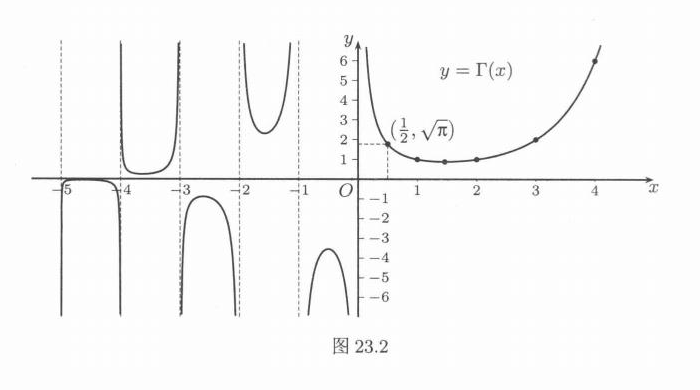
\includegraphics[width=.75\linewidth]{figures/lower/ch23/fig-23-2.png}
\end{center}
